\documentclass[master=ewit]{kulemt}
\setup{title={Newton-type operator splitting methods for embedded model predictive control},
  author={Willem Melis},
  promotor={Prof.\,dr.\,ir.\ Panagiotis Patrinos},
  assessor={Prof.\,dr.\,ir.\ Johan Suykens \\ Prof.\,dr.\,ir.\ Daan Huybrechs},
  assistant={dr.\,Pantelis Sopasakis}}
% The following \setup may be removed entirely if no filing card is wanted
\setup{filingcard,
  translatedtitle=,
  udc=621.3,
  shortabstract={TODO: Add the same abstract here, containing no more than 500
    words. \LaTeX\ commands can be used here. Blank lines (or the command
    \texttt{\string\pa r}) are not allowed!
    \endgraf endgraf}}
% Uncomment the next line for generating the cover page
% \setup{coverpageonly}

\setup{filingcard, % Do not change anything in this line!
	%
	% Give the dutch translation of the title of your master's thesis below between the { and }:
	translatedtitle={Newton-type operator splitsen methoden voor embedded model predictive control},
	%
	% UDC number depends on your discipline. see http://www.udcsummary.info/php/index.php to find the number.
	udc=621.3,
	%
	% Add between { and } a short abstract.
	% Empty lines or the commando \par are not admitted.
	% Be careful with special TeX-signs #$%&^_~{}\ !!
	shortabstract={%
    The goal of this thesis is to implement a Matlab and Python library that generates a MPC controller in C that makes use of the PANOC algorithm. No toolboxes or external libraries were used to generated the C code, with the  exception of Casadi. Casadi is used to generate the gradient used in the proximal gradient algorithm. In the first chapters the PANOC algorithm is discussed. Followed by a high level view of nmpc-codegen, the software package constructed with this thesis. After the theory some simulation results are included that compare PANOC to some of the state of the art interior point and SQP solvers. PANOC dominates the simulations when the system equations are small, but loses this advantage when complex system equations are used. It does however always use less memory then the alternatives. The final chapter discuses a recent improvement of the PANOC algorithm. When adding soft constraints onto the problem, the weights of theses constraints must be set. Setting the weights too low will result in violations of those constraints, and setting it too worsens the condition of the problem. Recent research surrounding PANOC and the augmented Lagrangian sudgest that by defining and solving the MPC problem iteratively, the performance can be significantly improved. It is also much more intuitive to tune the augmented Lagrangian then to tune the weights of the constraints.	
}}

% Choose the main text font (e.g., Latin Modern)
\setup{font=lm}

\bibliographystyle{IEEEtran}

\usepackage{algorithm} 
\usepackage{algcompatible}
\usepackage{algpseudocode}
%\usepackage[parfill]{parskip} % paragraphs are seperated with an enter space

% Finally the hyperref package is used for pdf files.
% This can be commented out for printed versions.
\usepackage[pdfusetitle,colorlinks,plainpages=false]{hyperref}

\usepackage{graphicx}
\graphicspath{{./figs/}}
\usepackage{caption}
\usepackage{subcaption}
\usepackage{amssymb}
\usepackage{listings}
\usepackage{tabularx}

% package used to import poster
\usepackage[final]{pdfpages}

\usepackage{amsmath,amsthm,amssymb}
\DeclareMathOperator{\project}{project}
\DeclareMathOperator{\prox}{prox}
\DeclareMathOperator{\boxfunction}{box}
\DeclareMathOperator{\argmax}{argmax}
\DeclareMathOperator*{\minimize}{minimize}
\DeclareMathOperator*{\argmin}{arg\,min}
\DeclareMathOperator{\other}{other}

\newcommand{\Lagr}{\mathcal{L}} % this uses the amssym package

%\includeonly{chap-n}
\begin{document}

\begin{preface}
I would like to thank everyone that contributed in any way to this thesis, especially my promoter P. Patrinos and mentor P. Sopasakis. I would also like to thank the jury for reading the text. Finally i would like to thank my family for the moral support they gave me this last year.
\end{preface}

\tableofcontents*

\begin{abstract}
  The \texttt{abstract} environment contains a more extensive overview of
  the work. But it should be limited to one page.

\end{abstract}

% A list of figures and tables is optional
\listoffigures
\listoftables
% If you only have a few figures and tables you can use the following instead

% The list of symbols is also optional.
% This list must be created manually, e.g., as follows:
\chapter{List of Abbreviations and Symbols}
\section*{Abbreviations}
\begin{flushleft}
  \renewcommand{\arraystretch}{1.1}
  \begin{tabularx}{\textwidth}{@{}p{18mm}X@{}}
  	BFGS   		& Broyden Fletcher Goldfarb Shanno \\
   	L-BFGS   	& Limited memory Broyden Fletcher Goldfarb Shanno \\
   	MM     		& Majorization-minimization
  \end{tabularx}
\end{flushleft}
\section*{Symbols}
\begin{flushleft}
  \renewcommand{\arraystretch}{1.1}
  \begin{tabularx}{\textwidth}{@{}p{12mm}X@{}}
    $\min$    & minimize \\
    $\mathbb{R}$   & The set of rational numbers \\
    $\mathbb{N}$   & The set of natural numbers \\
    $\nabla f$     & Gradient of f \\
    $f_{\mu}$      & Moreau envelope of f \\
    $\sum$         & Sum \\
    $\prod$        & Product \\
    $\partial$     & Partial derivative \\
    $\Lagr $       & Lagrangian \\
    $\prox_{\gamma g}$ & Proximal mapping of function g \\
    $I_c$          & Indicator function of set C \\
  \end{tabularx}
\end{flushleft}

% Now comes the main text
\mainmatter

%\chapter{Introduction}
\label{cha:intro}
The first contains a general introduction to the work. The goals are
defined and the modus operandi is explained.

\section{Lorem Ipsum 4--5}
\lipsum[4-5]

\section{Lorem Ipsum 6--7}
\lipsum[6-7]

%%% Local Variables: 
%%% mode: latex
%%% TeX-master: "thesis"
%%% End: 

\chapter{Control Systems}
\section{Optimal control}
	The optimal control problem goes back more than 300 years. From Galileo and Newton to Johann Bernoulli and Euler with the brachistochrone problem. The optimal control problem can be simplified to finding the proper inputs so that the system behaves in a certain way, or put differently, find the control law.
	
	A typical optimal control problem exists out of a set of differential equations that describes the behavior of the system. And a cost function that describes the cost of the specific trajectory integrated on the differential equations. The most optimal solution to the optimal control problem will have the lowest cost possible.
	
	Optimal control problems can be mathematically defined as the cost function equation~\ref{eq:optimal control definition}(With boundary conditions equation~\ref{eq:optimal control definition state equations boundary conditions})  and the behavior of the system equation~\ref{eq:optimal control definition state equations}. In addition constraints can be placed on the state and inputs, as shown by equation~\ref{eq:optimal control definition state equations path constraints}. 
	
	\begin{equation}
		J = S[x(t_0),t_0,x(T),T] + \int_{t_0}^{T} L[x(t),u(t),t]
		\label{eq:optimal control definition}
	\end{equation}
	\begin{equation}
		\dot{x}(t) = F(x(t),u(t),t)
		\label{eq:optimal control definition state equations}
	\end{equation}
	\begin{equation}
		C[x(t),u(t),t]\le 0
		\label{eq:optimal control definition state equations path constraints}
	\end{equation}
	\begin{equation}
		S[x(t_0),t_0,x(T),T]=0
		\label{eq:optimal control definition state equations boundary conditions}
	\end{equation}

\section{MPC}
	Model predictive control is an advanced process control method that continuously solves a  optimal control problem. At a constant rate the state is measured, a optimal control problem is define and solved. The  optimal input is applied to the system, and the cycle repeats itself.
	
	A continuous physical system can be defined as $\dot{x}=F_c(x,u)$, where x is the current state and u is the current input. However when using computer systems its often required to have a discrete system. By using a discrete integrator the system can be written as $x^{k+1}=F_d(x^{k},u^{k})$. 
	
	Figure~\ref{fig:MPC diagram} is a diagram from \cite{Wikipedia} that illustrates MPC. The reference trajectory is the behavior we want, the predicted control input is the control input that was calculated and in the simulations lead to the predicted output.
	\begin{figure}[h]
		\centering
		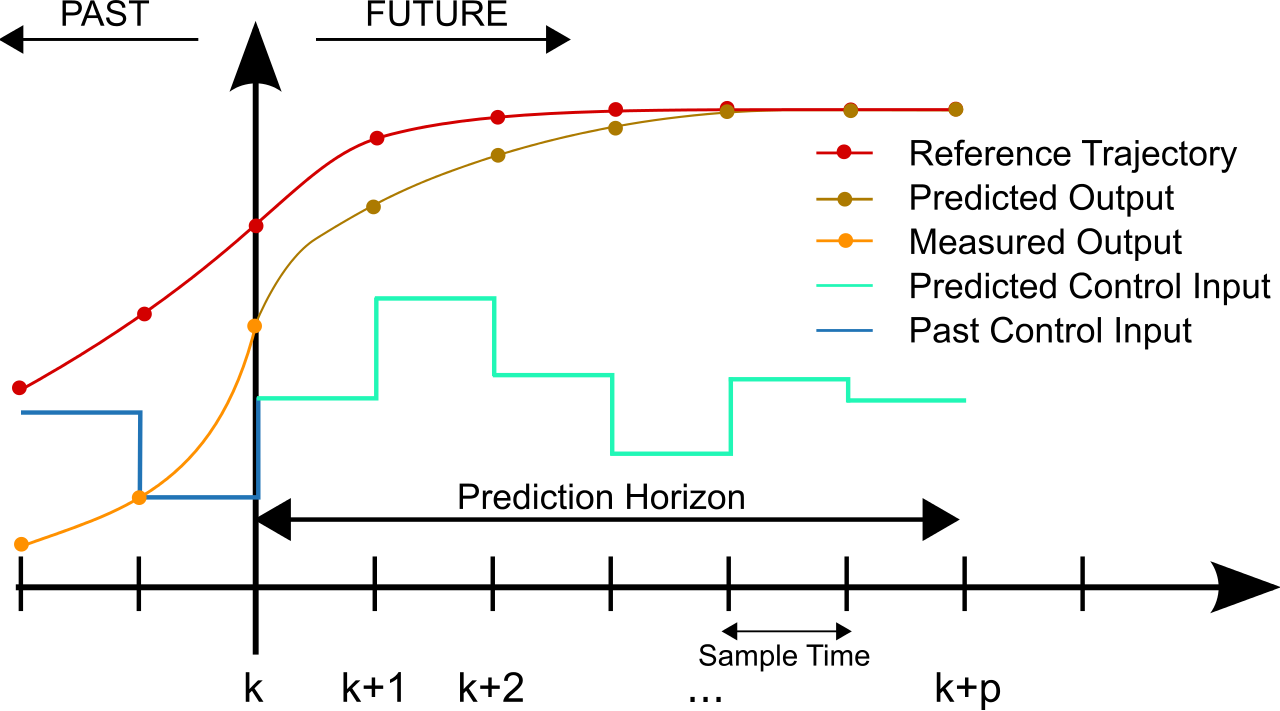
\includegraphics[width=0.5\textwidth]{MPC_scheme}
		\caption{A simple MPC diagram from the wikipedia page \cite{Wikipedia}}
		\label{fig:MPC diagram}
	\end{figure}
			
	\subsection{System}
		
	\subsection{Problem definition}
		\subsubsection{Problem form}
			The goal is to define the problem as equation~\ref{eq:PANOC MPC form}, and then solve it for u given $x_0$, the current state of the system. Sometimes $x_0$ will be assumed to be part of the function f, just like the reference state and input. Which leads to the simplified equation, equation~\ref{eq:PANOC form} .
			\begin{equation}
				\underset{u}{\minimize} \  f(x_0,u) + g(u)
				\label{eq:PANOC MPC form}
			\end{equation}
			
			\begin{equation}
				\underset{u}{\minimize} \  f(u) + g(u)
				\label{eq:PANOC form}
			\end{equation}
		\subsubsection{Direct Single shoot}
			If the horizon is N then the problem is solved for the inputs $u=[u_0,u_1,... u_{N-1}]$ where each $u_k$ is a vector of all the inputs of the system. This means that the vector u is of size Horizon $\cdot$ dimension\_input .
			
			The cost for each step in the horizon is defined as \ref{eq:single shot iteration cost}, this is called the stage cost.
			\begin{equation}
				\begin{aligned}
				& l_k(x_0,u) = &&  x_k^T Q x_k  +  u_k^T R u_k \\
				& \text{subject to}			&& x_0 = \bar{x} \\
				& 							&&  x_{n+1} = F_d(x_n,u_n), n=0...N-1
				\end{aligned}
				\label{eq:single shot iteration cost}
			\end{equation}
			
			The terminal cost is a special case of the stage cost as it is the last stage cost in the horizon. So if the Horizon=N the terminal cost can defined as equation~\ref{eq:single shot terminal cost}.
			
			\begin{equation}
				\begin{aligned}
					& l_N(x_0,u) = && x_N^TSx_N \\
					& \text{subject to}			&& x_0 = \bar{x} \\
					& 							&&  x_{n+1} = F_d(x_n,u_n), n=0...N-1
				\end{aligned}
				\label{eq:single shot terminal cost}
			\end{equation}
			
			$f(x_0,u)$ can then be defined as in equation~\ref{eq:single shot definition}, the sum of the stage costs and the terminal cost.
			\begin{equation}
				f(x_0,u) = \sum_{k=1}^{N-1} l_k(x_0,u) + l_N
				\label{eq:single shot definition}
			\end{equation}
			
			As a side note, an other term can be added to equation~\ref{eq:single shot definition} to represent the obstacle avoidance. More on this later on in this chapter in the subsection on obstacles.
		\subsection{Direct Multiple shoot}
			The multiple shoot needs more information than just an initial state. It requires an initial estimate of all of the intermediate states. The state estimates will be referred to as $x_i$ and the states derived from the estimate and its corresponding input will be referred to as $\bar{x_i}$. As before the goal of the optimization algorithm is to find the optimal inputs $u_i$, so that the cost function is as low as possible. And additionally  $\bar{x_i} - x_{i+1} = 0$, called the continuity conditions.
			
			\begin{equation}
				\bar{x_i} = F(x_i,u_i)
				\label{eq:}
			\end{equation}
			
			The continuity conditions are displayed in equation~\ref{eq:continuety condition multiple shot} and were not necessary in single shot as there are no state estimates like $\bar{x}$. If when starting the algorithm the initial state estimates are relatively close to the solution, a significant speed increase can be accomplished. As information was incorporate into the algorithm.
			
			\begin{equation}
				\bar{x_i} - x_{i+1} = 0
				\label{eq:continuety condition multiple shot}
			\end{equation}
			
			The direct multiple shoot definition looks like equation~\ref{eq:multiple shot cost} and has an extra equality condition compared to the single shoot. This equality condition will be added as a soft constraints to the cost function. This is displayed in equation~\ref{eq:multiple shot cost with soft constraint} and will be used in the practical implementation.
			
			\begin{equation}
				\begin{aligned}
				L =  & \sum_{i=1}^{N} l(\bar{x_i},u_i) \\
				& \text{subject to}			&& \bar{x_i} = F(x_i,u_i) \\
				& 							&& \bar{x_i} - x_{i+1} = 0
				\end{aligned}
				\label{eq:multiple shot cost}
			\end{equation}
			
			\begin{equation}
			\begin{aligned}
			L =  & \sum_{i=1}^{N} l(\bar{x_i},u) + ||\bar{x_i} - x_{i+1}||\\
			& \text{subject to}			&& \bar{x_i} = F(x_i,u_i) \\
			\end{aligned}
			\label{eq:multiple shot cost with soft constraint}
			\end{equation}
			
		\subsection{Obstacle avoidance}
			The obstacle avoidance is based on the soft constraint definition described in \cite{AjaySathya2017}. It can be described as a set or an constraint.
			\subsubsection{As set}
				An obstacle can be defined as an open set, as illustrated by equation~\ref{eq:obstacle as open set}. It is defined by the intersection of a set of nonlinear inequalities.
				\begin{equation}
					O = {z \in \Re^d : h^i(z)>0,\ i \in N}
					\label{eq:obstacle as open set}
				\end{equation}
				
			\subsubsection{As constraint}
				\begin{equation}
					[z]_+ =  \max\{0,z\}
				\end{equation}
				
				The statement $h(x)<0$ is equivalent to saying $[h(x)]_+=0$, so equation~\ref{eq:obstacle as open set} is equivalent to setting equation~\ref{eq:obstacle as equality} to zero.
				
				\begin{equation}
					\Phi_0(z) =  \frac{1}{2} \prod_{i=1}^m \Big( [h^i(z)]_+ \Big)^2
					\label{eq:obstacle as equality}
				\end{equation}
				
				The gradient of equation~\ref{eq:obstacle as equality} is define as equation~\ref{eq:obstacle as equality}
				
				\begin{equation}
					\nabla \Phi =
					\begin{cases}
						\sum_{i=1}^{m} h^i(z)\prod_{j \ne i} \Big( [h^i(z)]_+ \Big)^2 \nabla h^i(z)
						& x \in O \\
						0 & else
					\end{cases}
					\label{eq:derivative obstacle as equality}
				\end{equation}
			
			\subsubsection{Polyhedral obstacle}
				A simple obstacle example of such an obstacle is a polyhedral as defined in equation~\ref{eq:polyhedral constraint}.
				\begin{equation}
					\prod \Big([b_i - a_i^t z]_+ \Big)^2 = 0
					\label{eq:polyhedral constraint}
				\end{equation}
			
			\subsubsection{Obstacle as soft constraint}
				The obstacle avoidance is added as a soft constraint to the cost function. As demonstrated in equation~\ref{eq:derivative obstacle as equality}, this definition is two times differentiable and so this does not break the condition that the cost functions needs a gradient to be solved with the PANOC algorithm.
			
		\subsection{Input constraints}
			An other important aspect of a MPC problem are input constraints. In practice inputs have to comply with the physical properties of the devices. Absurdly high or low input values might in theory lead to a fast solution, but are not feasible in practice.
			
			A major advantage of the PANOC algorithm is that it can take non linear or non convex constraints. As longs as the proximal operation is analytically defined on the constraint it is feasible. 
			
			A simple example is the indicator box function, which allows to set a maximum and minimum value on the inputs. (The indicator box function is defined in the appendix) The indicator box function as input constraint can demand that every feasible solution lies within the bounds of the user defined box.
\chapter{Proximal gradient method}
	\subsection{Proximal mapping}
		The proximal operator is defined as $\prox_g(x)= \underset{u}{\argmin}(g(u) + \frac{1}{2 \gamma}||u-x||^2_2)$. 
		
		\begin{itemize}
			\item if $h(x)=0$ then $\prox_h(x)=x$ 
			\item if $h(x)=I_c(x)$ where $I_c$ is define in \eqref{eq:indicator function}, the proximity operator on an indicator function is the orthogonal projection on the set.
		\end{itemize}
		
		The indicator function: is defined in equation ~\eqref{eq:indicator function}.
		\begin{equation}
			I_c = 
			\begin{cases}
			0 & x \in C  \\
			\infty & x \notin C
			\end{cases}
			\label{eq:indicator function}
		\end{equation}
		
		The proximal mapping can be seen as a generalization of a projection. The Appendix contains an other important example, the indicator box function.
	
	\subsection{Gradient projected method}
		
		\begin{equation}
			\begin{aligned}
			& \underset{x}{\text{argmin}}
			& & f_0(x) \\
			& \text{subject to}
			& & g(x)=0
			\end{aligned}
			\label{eq:prox grad opti problem}
		\end{equation}
		
		The classical gradient decent method cannot be used to solve the problem of \eqref{eq:prox grad opti problem}. As this problem has a condition that must be met by the algorithms solution. If in each iteration the solution is projected on the space spanned by $g(x)=0$ the iteration \eqref{eq:grad descent} becomes \eqref{eq:projected grad descent}. This algorithm is called the gradient projection method.
		
		\begin{equation}
			x^k = x^{k-1} - \gamma \nabla f(x^{k-1})
			\label{eq:grad descent}
		\end{equation}
		
		\begin{equation}
			x^k = \project_{g(x)=0}[ x^{k-1} - \gamma \nabla f(x^{k-1})]
			\label{eq:projected grad descent}
		\end{equation}
		
		If $g(x)$ is the indicator function of the set onto which is projected. Then  \eqref{eq:projected grad descent} can be written as \eqref{eq:proximal grad descent}, known as the proximal gradient method.
		
		\begin{equation}
				x^k = \prox_{\gamma g}[ x^{k-1} - \gamma \nabla f(x^{k-1})]
			\label{eq:proximal grad descent}
		\end{equation}
	
	\subsection{The proximal gradient method}
		\eqref{eq:prox grad problem} Can be solved with the proximal gradient method, sometimes called forward backward splitting - FBS . Where the proximal mapping of $g(x)$ is analytically defined. 
			\begin{equation}
			\underset{x}{\argmin} = f(x) + g(x)
			\label{eq:prox grad problem}
			\end{equation}
		
		Inspired by the projected gradient method, the proximal gradient method is defined as \eqref{eq:prox grad method}. The $\gamma$ variable is the step size, in order to have a convergence of O(1/k) $\gamma \in(0,1/L)$. If $\gamma \in (1/L,2/L)$ the algorithm will still converge but then its no longer a majorization-minimization method. (more on this see \cite{NealParikh})
		
		\begin{equation}
			x^k = \prox_{\gamma g}\big( x^{(k-1)}- \gamma \nabla f(x^{(k-1)})\big)
			\label{eq:prox grad method}
		\end{equation}	
	
	\subsection{Proximal minimization algorithm}
		 \cite{QianYang} Contains a short proof that illustrates the proximal mapping as a fixed point minimization algorithm. A property of the conjugated function is used to derive the gradient, see appendix for the theorem.
		 \begin{proof}
		 	the iteration $x^{k+1}=\prox_g(x^k)$ will minimize the smoothed version of function f(x) 
		 	\begin{align*}
		 	f_{\mu}
		 	&= \underset{y}{\inf}\Big\{ |y| +\frac{1}{2 \mu}(x-y)^2 \Big\} \\
		 	&=   \frac{1}{2 \mu}||x||^2 + \frac{1}{2\mu} 
		 	\underset{y}{\inf}\Big\{
		 	2 \mu f(y) - 2x^T y + ||y||^2
		 	\Big\} \\
		 	&=  \frac{1}{2 \mu}||x||^2 + \frac{1}{\mu} 
		 	\underset{y}{\sup}\Big\{
		 	x^T y  - \mu f(y) - \frac{1}{2} ||y||^2 \Big \} \\
		 	&= \frac{1}{2\mu }||x||^2 \frac{1}{\mu } \Big( \mu f + \frac{1}{2}||\cdot||^2 \Big)^* (x) \\
		 	\nabla  f_{\mu} 
		 	&= \frac{x}{\mu} - \frac{1}{\mu} \underset{y}{\argmax} 
		 	\Big \{ x^Ty - \mu f(y) - \frac{1}{2}||y||^2 \Big \}\\
		 	& = \frac{1}{\mu}(x - \prox_{\mu f}(x)) \\
		 	\prox_{\mu f}(x)
		 	& = x- \mu \nabla f_{\mu}(x)
		 	\end{align*}
		 	\label{prf:proximal minimiztion alg proof}
		 \end{proof}

		 This means thats the iteration $x^{k+1}=\prox_g(x^k)$ will minimize the smoothed version of function g(x). 

\section{Proximal gradient method with line search}
	\subsection{Starting value gamma }
		\subsubsection{Estimating Lipschitz value}
			The Lipschitz of $\nabla f(x)$ value is a non negative number that complies with \eqref{eq:definition lipschitz value}.
			\begin{equation}
			L = \underset{x \neq y}{\sup} \frac{|\nabla f(y)-\nabla f(x)|}{|y-x|}
			\label{eq:definition lipschitz value}
			\end{equation}
			
			In practice it is not always possible to find the actual Lipschitz value. So the Lipschitz value is estimated ($L'$) locally at the starting location $x_0$ of the algorithm using \eqref{eq:estimated lipschitz value in starting position}. With $\delta=max[\delta_l,10^{-6} \cdot x_0]$ where $\delta_l$ is a small number chosen by the controller designer.
			% in code the safety value is DELTA_LIPSCHITZ_SAFETY_VALUE and set to 10^-6
			
			\begin{equation}
			L' = \frac{|\nabla f(x_0+\delta)-\nabla f(x_0)|}{|\delta|}
			\label{eq:estimated lipschitz value in starting position}
			\end{equation}
			
			The Lipschitz value is not explicitly saved but is used to estimate the line-search parameter $\gamma$. The backtracking of the proximal gradient descent then further improves this estimate. As the algorithm progresses and $\gamma$ improves, so does the estimation of the Lipschitz value indirectly.
		
		\subsubsection{Estimating gamma}	
			From \cite{LorenzoStella2017} it is known that $\gamma<\frac{1}{L}$ in order to guarantee convergence to a local minimum. As gamma needs to be smaller than $\frac{1}{L}$ a safety value is introduced. This idea was copied over from the kul-forbes/ForBES library by Lorenzo Stella and Panos Patrinos, which uses a $\beta$ of 0.05. And leads to \eqref{eq:starting value gamma}.
			\begin{equation}
			\gamma = \frac{1-\beta}{L}
			\label{eq:starting value gamma}
			\end{equation}		
	
	\subsection{Backtracking gamma}
		\subsubsection{Backtracking algorithm}
			Line-search is based on "Armijo's sufficient decrease condition" written down as \eqref{eq:Armijo's sufficient decrease condition}. The safety parameter $\theta$ multiplied with the step size $t_k$ is $\gamma=\theta \cdot t_k$. 
			
			\begin{equation}
			f(x_k + t_kp_k) \leq f(x_k) + \theta t_k \nabla f(x_k)^Tp_k
			\label{eq:Armijo's sufficient decrease condition}
			\end{equation}
			
			Line-search more specific backtracking will reduce the value of $\gamma$ until the condition of \eqref{eq:Armijo's sufficient decrease condition} fails.
			
		\subsubsection{Backtracking in proximal gradient descent used in FBS}
			The  "Armijo's sufficient decrease condition" is adjusted to \eqref{eq:Armijo's sufficient decrease condition prox grad PANOC} Which is an quadratic bound, $-p_k=x-\bar{x}$ and an additional term $\frac{1-\beta}{2 \gamma}||x-\bar{x}||^2$ is added.
			
			\begin{equation}
			f({\bar{x}}) \leq f(x) - \nabla f(x)^T[x-\bar{x}] + \frac{1}{2 \gamma}||x-\bar{x}||^2
			\label{eq:Armijo's sufficient decrease condition prox grad PANOC}
			\end{equation}
			
			This all leads to algorithm~\ref{alg:backtracking on gamma} the proximal gradient method. \eqref{eq:Armijo's sufficient decrease condition prox grad PANOC} can be seen as a quadratic model, as the Lipschitz value of the gradient is equal to $L=\frac{1}{\gamma}$.
			
			\begin{algorithm}
				\caption{backtracking $\gamma$}
				\label{alg:backtracking on gamma}
				\begin{algorithmic}[1]
					\Procedure {lineasearch\_gamma}{x,$\gamma$}
					\State $\bar{x} = \prox_{\gamma g}\big( x- \gamma \nabla f(x)\big)$
					\While{$f({\bar{x}}) > f(x) - \nabla f(x)^T[x-\bar{x}] + \frac{1}{2 \gamma}||x-\bar{x}||^2$}
					\State $\gamma = \frac{\gamma}{2}$
					\State $\bar{x} = \prox_{\gamma g}\big( x- \gamma \nabla f(x)\big)$
					\EndWhile
					\State \Return $\gamma$
					\EndProcedure
				\end{algorithmic}
			\end{algorithm}
	\subsection{Final algorthm}
		The final algorithm~\ref{alg:proximal gradient PANOC with backtracking} delivers the upward direction. $x_{k+1}=x_k - direction$.
		\begin{algorithm}
			\caption{proximal gradient PANOC with backtracking}
			\label{alg:proximal gradient PANOC with backtracking}
			\begin{algorithmic}[1]
				\Procedure{get\_proximal\_gradient\_step}{x,$\gamma$}
				\State $\gamma$=LINESEARCH\_GAMMA($\gamma$)
				\State $\bar{x} = \prox_{\gamma g}\big( x- \gamma \nabla f(x)\big)$
				\State \Return direction=$[x-\bar{x}]$, $\gamma$
				\EndProcedure
			\end{algorithmic}
		\end{algorithm}
\section{Proximal gradient alternative view}
	\subsection{Majorization-minimization algorithm}
	A Majorization-minimization algorithm, is a type of algorithm that minimizes a surrogate function. The surrogate function is a approximation of the actual problem. And needs to have the conditions described in \eqref{eq:MM algorithm conditions}, where h(x,y) is a surrogate function and f(x) is the actual problem. The problem described in \eqref{eq:MM algorithm formula step} is iteratively solved until convergence.
	\begin{equation}
		\begin{cases}
			h(x,x) = f(x) \\
			h(x,y) \leq f(x)
		\end{cases}
		\label{eq:MM algorithm conditions}
	\end{equation}
	
	\begin{equation}
		x_{k+1} = \argmin_y h(x_k,y)
		\label{eq:MM algorithm formula step}
	\end{equation}

	\subsection{The proximal gradient as majorization-minimization algorithm}
	The proximal gradient algorithm can be seen as a majorization-minimization algorithm. Its surrogate function is described in \eqref{eq:surrogate function}, proof~\ref{prf:proximal gradient as MM} illustrates how minimizing the surrogates function is equal as taking a step of the proximal gradient algorithm.
	
	\begin{equation}
		h(x,y) = f(x) + \nabla f(x)^T(x-y) + \frac{1}{2 \cdot \gamma}||x-y||^2_2
		\label{eq:surrogate function}
	\end{equation}
	
	\begin{proof}
		$h(x,y) = f(x) + \nabla f(x)^T(x-y) + \frac{1}{2 \cdot \gamma}||x-y||^2_2$ is the MM surugate function of proximal gradient algorithm. The gradient is set too zero and solved for y.
		\begin{align*}
		h(x,y)
		& = f(x) + \nabla f(x)^T(x-y) + \frac{1}{2 \cdot \gamma}||x-y||^2_2 \\
		\frac{\partial h(x,y)}{\partial y}
		& = 0 + \nabla f(x) + \frac{1}{2 \cdot \gamma} + \frac{1}{2 \cdot \gamma}\frac{\partial ||x-y||^2_2}{\partial y}  \\	
		\frac{\partial ||x-y||^2_2}{\partial y}
		& = \frac{\partial(x-y)^T(x-y)}{\partial y} = \frac{\partial(-2x^Ty + y^Ty)}{\partial y} = -2x+y \\
		\frac{\partial h(x,y)}{\partial y}
		& = \nabla f(x) - \frac{x}{\gamma} + \frac{y}{2 \gamma} = 0 \\
		0
		& = \gamma \nabla f(x) - x + \frac{y}{2} \\
		y & = \gamma \nabla f(x) - x
		\end{align*}
		\label{prf:proximal gradient as MM}
	\end{proof}
\chapter{PANOC algorithm}
	This section is based on \cite{LorenzoStella2017} and \cite{AjaySathya2017}, the difference is that this text is focused implementation. And so the formula's often look slightly different. The Forward backward envelop part is based on \cite{Themelis}, which contains a slightly different algorithm that also uses the Forward backward envelop.
	\section{Introducing panoc}
		The PANOC algorithm is an accelerated version of the proximal gradient descent. The direction  $x-\bar{x}$ is a combination of the proximal gradient algorithm and second direction that makes use of curvature information. This second direction will hopefully accelerate the convergence of the algorithm.
		
		\begin{equation}
		x_{k+1} = x_k + (1-\tau_k)\cdot (x-\bar{x}) + \tau_k d_k
		\end{equation}
		
		The new term $\tau_kd_k$ should accelerate the convergence if $\tau_k\neq0$. The step $d_k$ is calculated using a quasi-newton algorithm. As a quasi-newton algorithm uses curvature information of the cost function, it uses information not available to a gradient descent based method. 
		
		Furthermore it has a super linear convergence rate when it gets close to the solution. Which is much faster then the sub-linear convergence of a gradient descent algorithm . On top of that, the quasi-newton method will not require extra function evaluations. Which are the major contributors to the costs of the algorithm.
		
	\section{Quasi newton method}
		\subsubsection{Problem definition}
			The iteration of equation~\ref{eq:prox grad method} can indirectly be used to solve the optimization problem.  By using the residue defined in equation~\ref{eq:residue prox grad method} a fixed point can be found. 
			
			\begin{equation}
			R_{\gamma}(x)= \frac{1}{\gamma}\left[ x - \prox_g( x - \nabla f(x)\gamma) \right]
			\label{eq:residue prox grad method}
			\end{equation}
			
			The solution of equation~\ref{eq:residue prox grad method} can be found trough the Newton iteration of equation~\ref{eq:newton iteration residual}. Where $H_k$ satisfies the inverse secant condition of equation~\ref{eq:newton iteration residual inverse secant}. As the implementation is aimed at embedded software a good option to solve this would be L-BFGS. More on this in the chapter on L-BFGS.
			
			\begin{equation}
			x^{k+1} = x^k -H_kR_{\gamma}(x^k)
			\label{eq:newton iteration residual}
			\end{equation}
			\begin{equation}
			x^{k+1} - x^k = H_{K+1} \Big( R_{\gamma}(x^{k+1})- R_{\gamma}(x^k) \Big)
			\label{eq:newton iteration residual inverse secant}
			\end{equation}
		
	\section{Forward backward envelop}	
		Newton iterations only converge quickly when they are close to the solution. In order to get better global behavior a proper global strategy is required. The optimization problem is changed from $\varphi(x) = f(x) + g(x)$ to equation~\ref{eq:FBE definition using Moreau envelope}. This problem is smoother while it still has the same optimal solution.(proof see \cite{LorenzoStella2017} and \cite{Themelis}) The same $\gamma$ as with the proximal gradient should be used, notice how the FBE contains the line-search condition use in the proximal gradient. (more on the FBE in \cite{Themelis})
		
		The Moreau envelope is de define as \ref{eq:Moreau envelope}, this smooths the function, and has a close relationship with the proximal operator as illustrated earlier. Using simple algebra equation~\ref{eq:FBE definition using Moreau envelope} can be transformed into equation~\ref{eq:FBE definition using quadratic approximation}.(proof in Appendix) The solution $y$ of the infimum defined in equation~\ref{eq:FBE definition using quadratic approximation} is $\bar{x}$. Considering the close relationship between the Moreau envelope and the proximal operator (see more in \cite{Themelis}) this is to be expected.
		
		An alternative way to look the FBE is illustrated in \cite{AjaySathya2017}, where the problem can be seen as minimizing a quadratic approximation  $f(x) +  \nabla f(x)^T(y-x) + g(y) + \frac{1}{2 \gamma} ||x-y||^2  $ towards y in point x.  Remember that $L = \frac{1}{\gamma}$, with L being the Lipschitz constant of the gradient.
		
		\begin{equation}
			g^{\gamma} = \underset{y}{\inf} \big \{f(y)+\frac{1}{2 \cdot \gamma}||x-y||^2 \big \}
			\label{eq:Moreau envelope}
		\end{equation}
		
		\begin{equation}
		\varphi_{\gamma} = f(x) - \frac{\gamma}{2}||\nabla f(x)||^2 + g^{\gamma} \big(x-\gamma \nabla f(x) \big)
		\label{eq:FBE definition using Moreau envelope}
		\end{equation}
		
		\begin{equation}
		\varphi_{\gamma} =   f(x) + \underset{y}{\inf} \Big\{ \nabla f(x)^T(y-x) + g(y) + \frac{1}{2 \gamma} ||x-y||^2  \Big\}
		\label{eq:FBE definition using quadratic approximation}
		\end{equation}
		
		\begin{proof}
			The solution to the infimum of equation~\ref{eq:FBE definition using quadratic approximation} is y=$\bar{x}= \prox_g(x-\gamma \nabla f(x))$
			\begin{align*}
			\prox_g(\bar{x}) 
			&=\prox_g(x- \gamma \nabla f(x)) \\
			&= \underset{y}{\argmin} \Big \{ g(y) 
			+ \frac{1}{2 \gamma}||(y-x) + \gamma \nabla f(x)||^2 \Big \} \\
			&= \underset{y}{\argmin} \Big \{ g(y) 
			+ \frac{1}{2 \gamma} \big[||y-x||^2 + 2 \gamma \nabla f(x)^T(y-x) + ||\nabla f(x)||^2\gamma^2 \big] \Big \} \\
			&= \underset{y}{\argmin} \Big \{ g(y) 
			+ \frac{1}{2 \gamma} \big[||y-x||^2 + 2 \gamma \nabla f(x)^T(y-x)  \big] \Big \}\\
			&= \underset{y}{\argmin} \Big \{   \nabla f(x)^T(y-x)  + g(y) 
			+ \frac{1}{2 \gamma} ||y-x||^2  \Big  \}
			\end{align*}
			\label{prf:prox is solution to FBE inf}
		\end{proof}
		
		Equation~\ref{eq:practical implementation of FBE} is the practical implementation of the FBE. The parameter gamma is the line-search parameter used in the proximal gradient descent. The first 3 terms are the same as with the line-search on $\gamma$, the last term $g(\bar{x})$ is new and makes sure the solution complies with the constraint.
		
%		\cite{AjaySathya2017} has an excellent example to illustrate this.(figure~\ref{fig:FBE illustration}).
%		
		\begin{equation}
			\begin{aligned}	
				& \varphi(\gamma,x)= 
				&& f(x) - \nabla f(x)^T(x-\bar{x}) + \frac{1}{2 \gamma}||x-\bar{x}||^2  + g(\bar{x})
				\\
				& with 
				&&\bar{x} = \prox_g( x - \gamma\nabla f(x)) 
			\end{aligned} 
			\label{eq:practical implementation of FBE}
		\end{equation}
		
%		\begin{figure}[H]
%			\centering
%			\label{fig:FBE illustration}
%			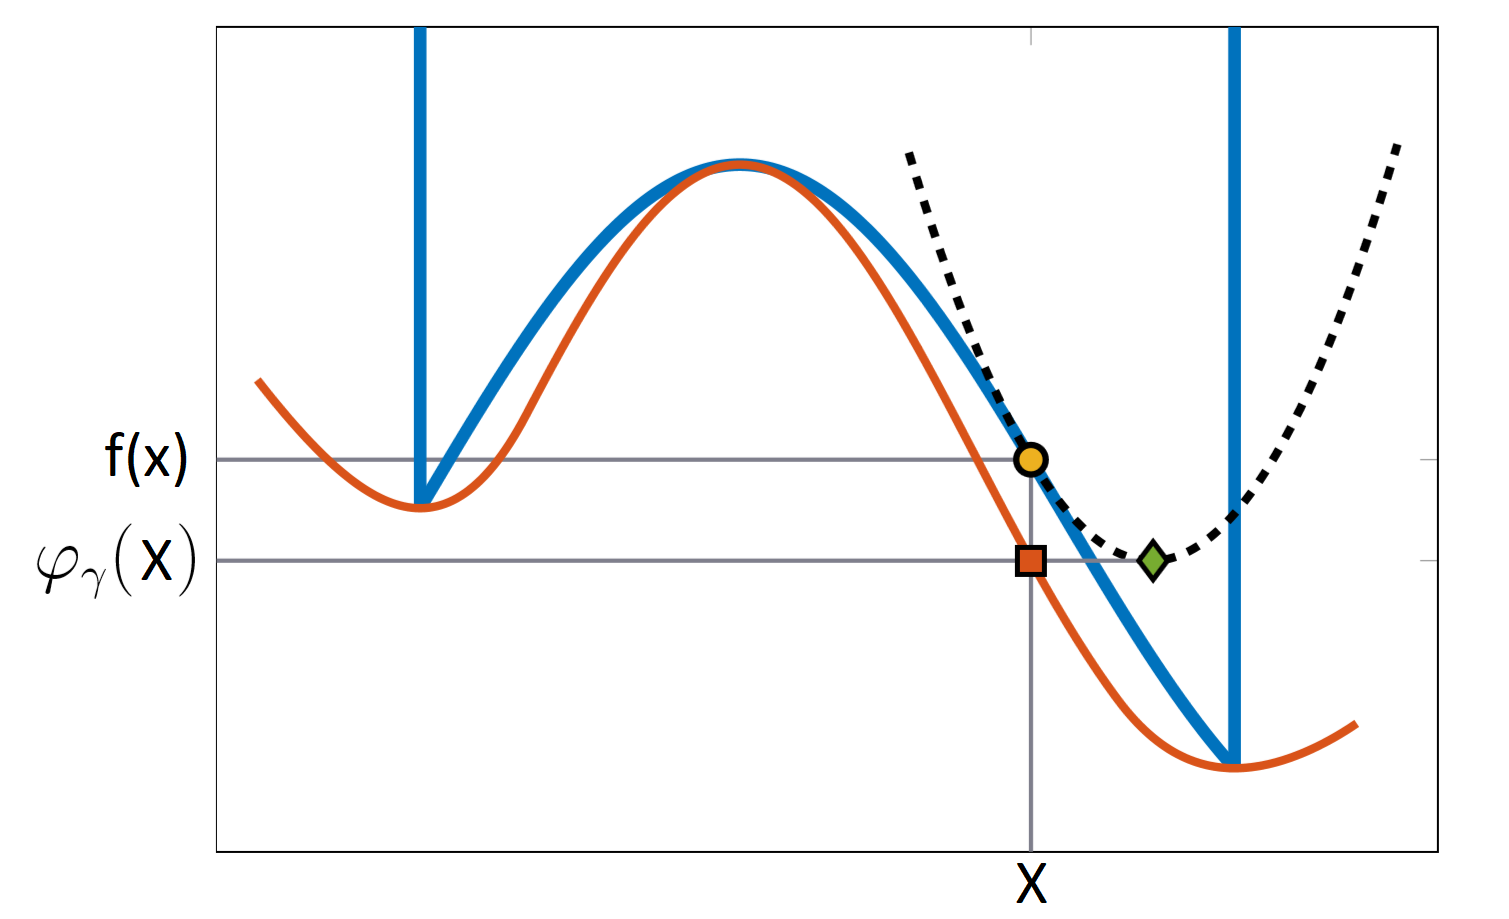
\includegraphics[width=0.6\textwidth]{FBE}
%			\caption{FBE example copied over from \cite{AjaySathya2017}, red is?? blue is ?? TODO expain this figure}
%		\end{figure}
	
	\section{Line-search with FBE}
	In \cite{LorenzoStella2017} the line-search condition is specified as equation ~\ref{eq:line-search with FBE}. The line-search parameter $\tau$ determines $x^{k+1}$ by choosing the convex combination of the step from the proximal gradient and the L-BGFS as defined in equation~\ref{eq:linea-search tau definition}.  \cite{LorenzoStella2017} specifies that $\sigma \in (0, \gamma \frac{1-\gamma\cdot L}{2})$. As stated before it is assumed that $L=\frac{1-\beta}{\gamma}$, some simple algebra will lead to the condition $\sigma \in (0,\frac{\beta \gamma}{2})$.
	
	 Equation~\ref{eq:practical line-search with FBE} is the practical implementation of equation~\ref{eq:line-search with FBE}. A new constant $\alpha \in (0,1)$ is introduced, an possible value for $\alpha$ would be 0.5 ($\alpha=0.5$ is the choice used by the Matlab implementation of PANOC in ForBes known as zerofpr2).
	
	\begin{equation}
		x^{k+1} = u_k - (1-\tau_k)\cdot (x-\bar{x}) + \tau \cdot dir_{LBFGS}
		\label{eq:linea-search tau definition}
	\end{equation}
	
	\begin{eqnarray}
		\label{eq:line-search with FBE}
		\varphi_{\gamma}(x^{k+1})\leq\varphi_{\gamma}(x^{k}) - \sigma ||\frac{x-\bar{x}}{\gamma}||^2 \\
		=
		\varphi_{\gamma}(x^{k}) - \frac{\sigma}{\gamma^2} ||x-\bar{x}||^2
	\end{eqnarray}
	
	\begin{equation}
		\varphi_{\gamma}(x^{k+1}) \leq 		\varphi_{\gamma}(x^{k}) - \alpha \frac{\beta }{\gamma \cdot 2} ||x-\bar{x}||^2
		\label{eq:practical line-search with FBE}
	\end{equation}
	
	
		
		\begin{algorithm}
			\caption{PANOC}
			\label{alg:PANOC}
			\begin{algorithmic}[1]
				\Procedure {PANOC\_GET\_NEW\_LOCATION}{$x^k$,$\gamma$}
				\State [$(x-\bar{x})$ , $\gamma$] = GET\_PROXIMAL\_GRADIENT\_STEP($\gamma$,$x^k$)
				\State $ dir_{LBFGS}$ = LBFGS($x^k$)
				\State $\tau =1$
				\State $x^{k+1} = x_k - (1-\tau_k)\cdot (x-\bar{x}) + \tau \cdot dir_{LBFGS}$
				\While{$\varphi_{\gamma}(x^{k+1}) > 		\varphi_{\gamma}(x^{k}) - \alpha \frac{\beta}{\gamma \cdot 2} ||(x-\bar{x})||^2$}
				\State $\tau = \tau / 2$
				\State $x^{k+1} = x_k - (1-\tau_k)\cdot (x-\bar{x}) + \tau \cdot dir_{LBFGS}$
				\EndWhile
				\EndProcedure
			\end{algorithmic}
		\end{algorithm}
	
\chapter{L-BFGS}
	In this chapter the implementation of solving \eqref{eq:LBFGS problem} with L-BFGS is discussed. A naive implementation can lead to strange behavior. So it's important to spend time on the L-BFGS implementation.
	
	
	\begin{equation}
	R(x) = \frac{1}{\gamma}\left[ x - \prox_g( x - \nabla f(x)\gamma) \right] = 0
	\label{eq:LBFGS problem}
	\end{equation}
	
	\section{Exact newton method}
	The exact Newton method can be derived from a Taylor expansion. Its quadratic convergence makes it a popular choice for solving optimization problems. However convergence is not guaranteed and only quadratic if it is close enough to the solution. The Hessian matrix must be available to the algorithm, and is used in each iteration of the algorithm to solve a system.
	
		\begin{equation}
			g(x_{k+1}) = g(x_k) + \nabla g(x_k)(x_{k+1}-x_k)
			\label{eq:Taylor expansion}
		\end{equation}
		
		\begin{equation}
			x_{k+1}-x_k = -(\nabla g(x_k))^{-1} \cdot g(x_k)
			\label{eq:Taylor expansion reshaped}
		\end{equation}
		
	The Taylor expansion in point $x^k$ can be written as \eqref{eq:Taylor expansion}, if $g(x^{k+1})$ is set to zero, the equation becomes \eqref{eq:Taylor expansion reshaped}. This leads to \eqref{eq:newton method} where $g(x)=\nabla f(x)$ and the step towards zero is p. Typically some sort of line search used to accelerate convergence, so the next location is found using \eqref{eq:newton method linesearch}, with linesearch parameter $\alpha$.	
	
		\begin{equation}
			p = x_{k+1}-x_k = -(\nabla^2 f(x_k))^{-1} \cdot \nabla f(x_k)
			\label{eq:newton method}	
		\end{equation}
	
		\begin{equation}
		 	x_{k+1} = x_k + \alpha p
		 	\label{eq:newton method linesearch}
		\end{equation}
		
	\section{Quasi Newton Method:BFGS}
	As mentioned in the previous section in order to use the exact Newton method the hessian matrix must be available in practice. Sometimes this matrix exists but is not analytically available. It might be hard to express analytically, or too large to save explicitly in memory. In either case it is possible to approximate the Hessian matrix as illustrated in \eqref{eq:quasi newton method approx Hessian}.  This leads to the secant condition \eqref{eq:secant condition}. One popular formulation that satisfies the secant condition is the BFGS algorithm.
		
		\begin{equation}
			B_{k+1}(x_{k+1}-x_k) = \nabla f(x_{k+1}) - \nabla f(x_k)
			\label{eq:quasi newton method approx Hessian}	
		\end{equation}
		
		\begin{eqnarray}
			s_k = x_{k+1} - x_{k} \\
			y_k = \nabla f(x_{k+1}) - \nabla f(x_{k}) \\
			\rho_k = \frac{1}{y_k^T \cdot s_k}
		\end{eqnarray}
	
		
		\begin{equation}
			B_{k+1} s_{k} = y_{k}
			\label{eq:secant condition}
		\end{equation}
		
		\begin{equation}
			B_{k+1} = B_{k} + \frac{y_k y_k^T}{ y_k^T s_k} - \frac{B_k s_k s_k^T B_k^T}{s_k^TB_ks_k}
			\label{eq:quasi newton method approx Hessian with past values}
		\end{equation}
	Calculating the inverse of the B matrix is an expensive operation. Solving a system of linear equations has a computational complexity of $\mathcal{O}(n)^3$ . According to \cite{Wright} \eqref{eq:quasi newton method inverse hessian} expresses the inverse of the Hessian in a function of the past values. In every iteration the L-BFGS step is calculated using \eqref{eq:quasi newton method}. The new location can now be used to update the inverse hessian using \eqref{eq:quasi newton method inverse hessian}.
		\begin{equation}
			V_k = I - \rho_ky_ks_k^T
		\end{equation}
	
		\begin{equation}
			H^{k+1} = V_k^TH_kV_k + \rho_ks_ks_k^T
			\label{eq:quasi newton method inverse hessian}	
		\end{equation}
		
		\begin{equation}
		p = x_{k+1}-x_k = -(B_k)^{-1} \cdot \nabla f(x_k) = -H_k\cdot \nabla f(x_k)
		\label{eq:quasi newton method}	
		\end{equation}
		
	\section{Quasi Newton Method:L-BGFS}
	One variation of the BFGS algorithm is the L-BFGS algorithm as described by \cite{Wright}. The L-BFGS algorithm does not express the Hessian matrix explicitly. This way less memory is required to run the algorithm. Which is very useful if either the problem is large, or the memory is small. As nmpc-codegen is aimed at embedded devices the latter is very important.
	
	\cite{Wright} States that \eqref{eq:quasi newton method inverse hessian} can be expressed recursively as \eqref{eq:quasi newton method inverse hessian recursive}. \eqref{eq:quasi newton method inverse hessian recursive} Can also be expressed in two loops as illustrated in algorithm~\ref{alg:LBFGS}.
	
		\begin{eqnarray}	 
			\begin{aligned}
				H_k = 
				& (V^T_{k-1} ... V^T_{k-m})H^0_k(V^T_{k-m} ... V_{k-1}) \\
				& + \rho_{k-m} (V^T_{k-1} ... V^T_{k-m+1})s_{k-m}s_{k-m}^T(V^T_{k-m+1} ... V_{k-1}) \\
				& + \rho_{k-m+1} (V^T_{k-1} ... V^T_{k-m+2})s_{k-m+1}s_{k-m+1}^T(V^T_{k-m+2} ... V_{k-1}) \\
				& + ... \\
				& + \rho_{k-1}s_{k-1}s_{k-1}^T
			\end{aligned}
			\label{eq:quasi newton method inverse hessian recursive}
		\end{eqnarray}
		
		\begin{equation}
			H_k^0 = \frac{s_k^Ty_k}{y_k^Ty_k}
			\label{eq:quasi newton method initial Hessian}
		\end{equation}
		
	The initial Hessian $H^0_k$ can be estimated using the most recent s and y values, as illustrated in \eqref{eq:quasi newton method initial Hessian}. If the optimal point is a local minimum, it's advisable to check if the new initial Hessian is positive definite. The next location then becomes $x_{k+1} = x_{k}+ \alpha \cdot p$ with alpha being the line search parameter. Typically either a wolf-type or Armijo-type line search is used, however PANOC uses neither of these methods so they are not discussed.
	
	\section{Cautious update L-BGFS}
	As mentioned before when updating the initial hessian value, it's good practice to check if it's positive. If it is negative, there's no point in updating the Hessian value. However even with this safety mechanism, it is still possible to get bad updates. As in updates that lower the convergence rate of future L-BFGS steps.
	
	\begin{equation}
		\frac{y_k^Ts_k}{s_k^Ts_k} \ge \epsilon ||\nabla f(x_k)||^\alpha
		\label{eq:cautious update}
	\end{equation}
	
	\cite{Dong-HuiLi1999} Suggests a cautious update based on the size of the gradient and $\frac{y_k^Ts_k}{s_k^Ts_k}$ as illustrated in \eqref{eq:cautious update}. The two parameters epsilon and alpha are both positive constants. The cautious update of \eqref{eq:cautious update} is relevant when the algorithm is near fixed point. And the step size is so small the function values hardly change. The information in $s_k$ and $y_k$ is then dominated by noise and cannot be trusted.
	
	\subsection{L-BFGS implementation}
		When using  L-BFGS algorithm(algorithm~\ref{alg:LBFGS}) to solve \eqref{eq:LBFGS problem}. The direction is equal to the proximal gradient step if there is no initial hessian estimate. The buffer size will increase with every valid update from 1 to the limit specified by the controller designer.
		
		\begin{equation}
			R(x) = \frac{1}{\gamma}\left[ x - \prox_g( x - \nabla f(x)\gamma) \right] = 0
			\tag{\eqref{eq:LBFGS problem} revisited}
		\end{equation}
		
		\begin{algorithm}
			\caption{LBFGS}
			\label{alg:LBFGS}
			\begin{algorithmic}[1]
				\Procedure {LBFGS}{$x^k$,M=current\_buffersize}
				\State $q = R(x^k)$
				\For{i=M:1}
				\State $\alpha(i)=\rho(i) \cdot s(:,i)^Tq$
				\State $q = q - \alpha(i) \cdot y(:,i)$
				\EndFor
				\State $H_k^0 = y(:,M) \cdot s(:,M)^T \cdot  \frac{1}{y(:,M)^T \cdot y(:,M)}$
				\State $H^0_k \cdot R(x^k)$
				\For{i=1:M}
				\State $\beta(i) = \rho(i) \cdot y(:,i)^T \cdot z$
				\State $z = z + s(:,i)[\alpha(i)-\beta(i)]$
				\EndFor
				\For{i=1:M-1}
				\State $s(:,i+1)=s(:,i)$
				\State $y(:,i+1)=y(:,i)$
				\EndFor
				\State $$\begin{cases}
				s(:,1) = x_{k+1} - x_k \\
				y(:,1) = \nabla f(x_{k+1}) - \nabla f(x_k)\\
				\rho_k(1) = \frac{1}{y(:,1)^T \cdot s(:,1)} \\ 
				\end{cases}
				$$
				\State \Return direction=$-z=-H_k \cdot R(x^k)$
				\EndProcedure
			\end{algorithmic}
		\end{algorithm}
	
	\subsection{Notes on implementing L-BFGS with PANOC}
	Even though the papers on the PANOC algorithm sudgest that the problem solved with L-BFGS is \eqref{eq:LBFGS problem}. Using the unnormalized $R'(x) = \left[ x - \prox_g( x - \nabla f(x)\gamma) \right]$ with the L-BFGS will give better numerical results.
	
	\begin{equation}
	R(x) = \frac{1}{\gamma}\left[ x - \prox_g( x - \nabla f(x)\gamma) \right] = 0
	\tag{\eqref{eq:LBFGS problem} revisited}
	\end{equation}
	
	Every time the search parameter $\gamma$ changes the L-BFGS buffer must be flushed.
\chapter{Nmpc-codegen}
This chapter describes the software library that was written for this thesis. First an overview of the workflow and the functionality of the library is given. Followed by a in-depth description of the implementation.
\section{Overview library}
The nmpc-codegen library contains a framework to construct a Python script that generates a MPC controller. This controller uses the panoc algorithm to solve the optimization problem.

Figure~\ref{fig:nmpc-codegen scheme} illustrates how this is accomplished. On the left side is the Python or Matlab script that the user will construct. It contains the mathematical model nd the control parameters of the process that needs to be controlled.The output of the Python script is displayed on the right side in figure~\ref{nmpc-codegen scheme}. The output contains some static code, which is mostly associated with the panoc algorithm. And some dynamic code which is generated in Python and will differ from problem to problem. Finally sometimes the output will also contain simulation tools, this optional feature allows the user to simulate the controller from within Python or Matlab.
	\begin{figure}[H]
		\centering
		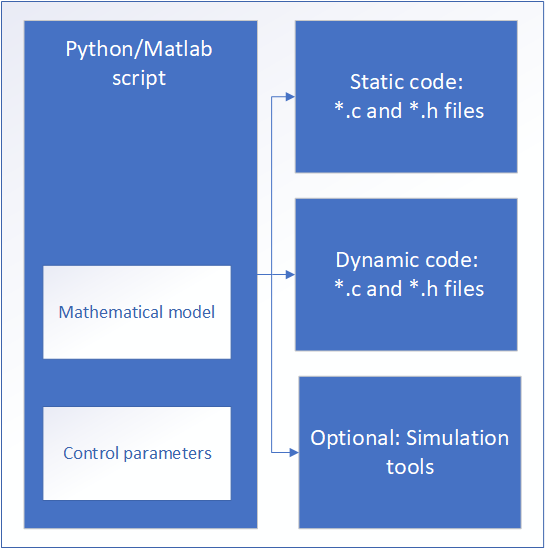
\includegraphics[width=0.5\textwidth]{nmpc_codegen_scheme}
		\caption{nmpc-codegen scheme}
		\label{fig:nmpc-codegen scheme}
	\end{figure}

\section{Casadi}
The panoc algorithm is a derivative driven algorithm, this means that the gradient of the cost function must be available to the algorithm. This gradient is generated using backward automatic differentiation.

\subsection{Algorithmic differentiation (AD)}
There exists a number of ways to determine the derivative of a function. The most obvious way is using symbolic differentiation. This method has been used over more than 200 years to calculate the gradient by hand. But in order to use symbolic differentiation, the algorithm needs one mathematical defined function. Which might be hard to get.

Another way of calculating derivatives, is through numerical differentiation also known as the method of finite differences. Although this method is very simple to implement, the accuracy is not always sufficient. And the method is rather slow if there are lots of partial derivatives.

An second alternative way to calculate the derivatives is through automatic differentiation. This method has two variants forward automatic differentiation and backward automatic differentiation.

The simplest of the two is forward differentiation, the only requirement to use this algorithm is that the entire function must be expressed in elementary operations. This is something computers are naturally good at. Equation~\ref{eq:example used with automatic differentiation} illustrates a simple example of such function. Two intermediate valuables are used to express the elementary operations.
\begin{equation}
	\begin{aligned}
		& y = a \cdot b + cos(b) \\
		& x_1 = a \cdot b \\
		& x_2 = cos(b) \\
		& y = x_1 + x_2		
	\end{aligned}
	\label{eq:example used with automatic differentiation}
\end{equation}
Forward automatic differentiation gets its name from the fact that the chain rule is applied from input to output. It derives from the lowest variables to the highest viable. As illustrated by equation~\ref{eq:math definition forward automatic differentation}. Equation~\ref{eq:example forward automatic differentiation} contains a worked out example of this algorithm. The first line of equation~\ref{eq:example forward automatic differentiation} contains the theoretical answer. The  following two lines contain the derivatives of the intermediate variables towards the b variable. Finally the to the derivatives are summed up and deserved it towards b is found.

The problem with forward automatic differentiation is that for each variable all the intermediate derivatives needs to be calculated. This is where the idea for backward automatic differentiation came from. As it allows to generate the derivative to all inputs variables in one big sweep. Although it's more expensive to calculate one single derivative, it is cheaper to calculate all the derivatives.

\begin{equation}
	\frac{dx_i}{db} = \frac{dx_i}{dx_j}\frac{dx_j}{dx_k}\frac{dx_k}{db}
	\label{eq:math definition forward automatic differentation}
\end{equation}

\begin{equation}
	\begin{aligned}
		& \frac{\partial y}{\partial b} = a - sin(b) \\
		& \frac{\partial x_1}{\partial b} = a  \\
		& \frac{\partial x_2}{\partial b} = -sin(b) \\
		& \frac{\partial y}{\partial b} = \frac{\partial x_1}{\partial b} + \frac{\partial x_2}{\partial b}	 = a - sin(b)
	\end{aligned}
	\label{eq:example forward automatic differentiation}
\end{equation}

Backward automatic differentiation is the opposite of forward automatic differentiation as it works down from the output towards the input. As illustrated by equation~\ref{eq:math definition backward automatic differentation}. An example is worked out in equation~\ref{eq:example backward automatic differentiation}. Even if there are hundreds of intermediate variables it only required one line to find a component of the gradient. This is the main reason why packages like casadi use backward automatic differential, instead of forward.

\begin{equation}
	\frac{\partial x_i}{\partial b} = \frac{\partial x_i}{\partial x_k}\frac{\partial x_k}{\partial x_j}\frac{\partial x_j}{\partial b}
	\label{eq:math definition backward automatic differentation}
\end{equation}

\begin{equation}
\begin{aligned}
& \bar{x_1} = \bar{x_3} \frac{\partial x_3}{\partial x_1} = 1 \cdot 1 \\
& \bar{x_2} = \bar{x_3} \frac{\partial x_3}{\partial x_2} = 1 \cdot 1 \\
& \frac{\partial y}{\partial b} = \bar{x_1} \frac{\partial x_1}{\partial b} + \bar{x_2} \frac{\partial x_2}{\partial b} = a - sin(b)\\
& \frac{\partial y}{\partial a} = \bar{x_1} \frac{\partial x_1}{\partial a} = b
\end{aligned}
\label{eq:example backward automatic differentiation}
\end{equation}

The same example can be calculated with Casadi as demonstrated in listing~\ref{lst:casadi demo backward automatic differentiation} with output in table~\ref{tbl:output casadi demo backward automatic differentiation}. The intermediate variables are @1,@2 and @3. output[0][0] is the function value and input[1][0] and input[1][1] is the gradient. 

\begin{lstlisting}[caption={Casadi example automatic backward differentiation},label={lst:casadi demo backward automatic differentiation}]
a = cd.SX.sym('a',(1,1))
b = cd.SX.sym('b',(1,1))
y = a*b + cd.cos(b)
f = cd.Function('f',[a,b],[y,cd.gradient(y,cd.vertcat(a,b))])
print(f)
\end{lstlisting}


\begin{table}
	\begin{center}
		\begin{tabular}{ |l|  }
			\hline
			Output Casadi code listing~\ref{lst:casadi demo backward automatic differentiation} \\
			\hline
			Number of inputs: 2 \\
			Input 0 ("i0"): 1-by-1 (dense) \\
			Input 1 ("i1"): 1-by-1 (dense) \\
			Number of outputs: 2 \\
			Output 0 ("o0"): 1-by-1 (dense) \\
			Output 1 ("o1"): 2-by-1 (dense) \\
			@0 = input[0][0]; \\
			@1 = input[1][0]; \\
			@2 = (@0*@1); \\
			@3 = cos(@1); \\
			@2 = (@2+@3); \\
			output[0][0] = @2; \\
			output[1][0] = @1; \\
			@1 = sin(@1); \\
			@0 = (@0-@1); \\
			output[1][1] = @0; \\
			\hline   
		\end{tabular}
		\label{tbl:output casadi demo backward automatic differentiation}
	\end{center}
\end{table}



\section{Nmpc-codegen implementation}
Nmpc-codegen exists out of a high-level language such as Python or Matlab that generates header files and source files. In order to test the controller, the higher-level language can call the build system (Cmake/make) to compile the generate code. And then simulate the controller to see the response. At the end of the development cycle the Python/Matlab code can generate a clean controller without this build system.

\subsection{Python and Matlab}
Figure~\ref{fig:nmpc_codegen_packages} Illustrates the architecture of the nmpc-codegen library. There are five sub packages tools, models, example models, controller and Cfunctions.  The two classes in the sub package models, represent the mathematical model of the system. The user must construct an object of one of these classes, that contains the function equation of the system.

The Cfunctions sub package contains proximal functions that represent constraints on the inputs. The user manual contains a table of all available constraints to the user. The tools sub package contains two classes. The bootstrapper that can generate the static code, and the simulator that allows the user to call the generated C code from Python or Matlab.

The controller sub package contains the Nmpc\_panoc class, an object of this class represents the actual controller. In order to construct an object of the Nmpc\_panoc class the user must provide a model object, a proximal function object and one or two stage costs object.

Finally the user can also add obstacles, these will be added a soft constraints into the cost function. The obstacles can be found in the sub package obstacles from the sub package controller.
	\begin{figure}[H]
		\centering
		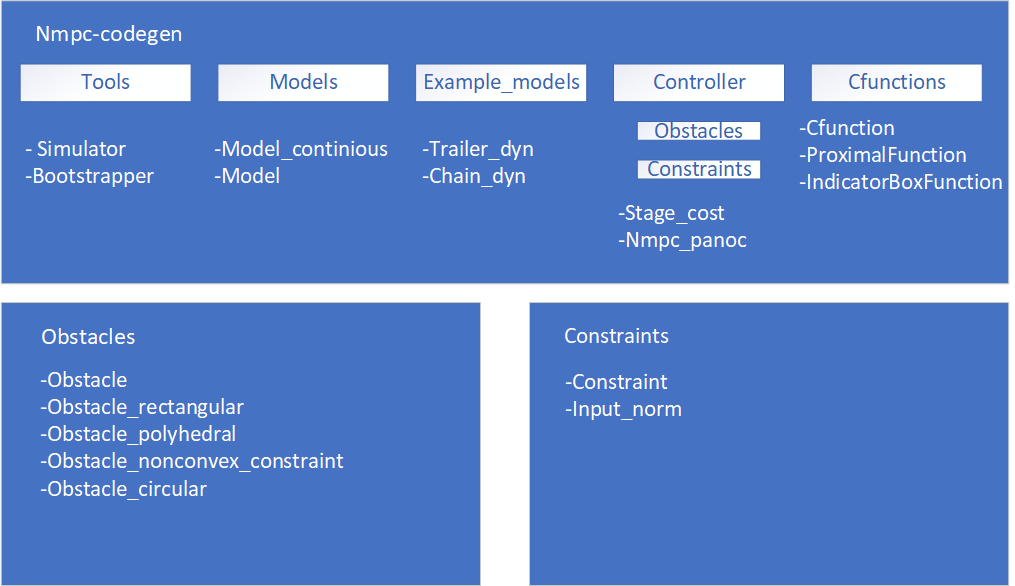
\includegraphics[width=1\textwidth]{nmpc_codegen_packages}
		\caption{Software architecture}
		\label{fig:nmpc_codegen_packages}
	\end{figure}

\subsection{C}
The C code is written in a layered architecture, the lowest layer contains the buffer, the cost function and the lipschitz estimator. The second layer contains the proximal gradient algorithm and the L-BFGS algorithm. The highest layer contains the panoc algorithm.

The NMPC entity initializes the cost function with the current state of each iteration, and calls panoc repeatably till convergence. The end-user does not need to know how panoc or any of the underlying layers work. The NMPC entity takes care of everything, the user will simply call NMPC with the current state, a reference state, a reference input and output array to place the optimal inputs.

	\begin{figure}[H]
		\centering
		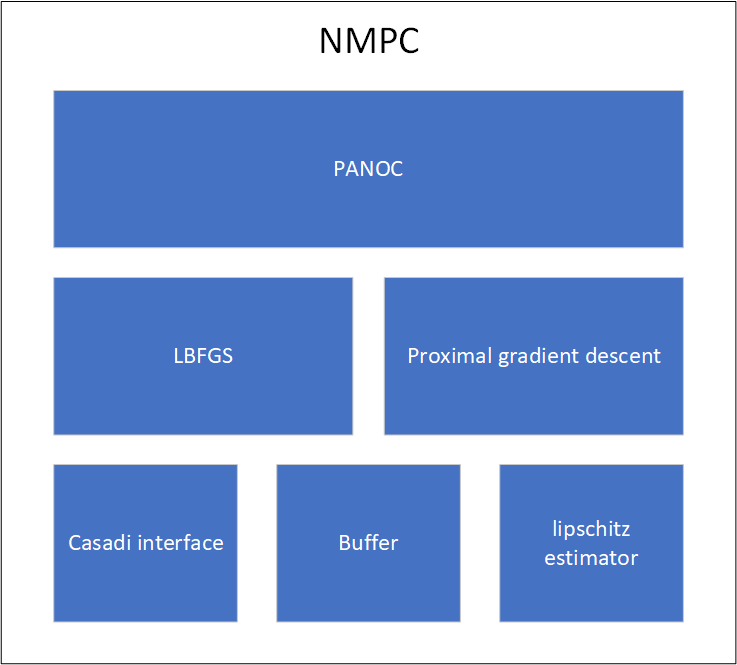
\includegraphics[width=0.5\textwidth]{visio_software_arch}
		\caption{Software architecture}
		\label{fig:visio software arch}
	\end{figure}

\subsection{Build system}
The build system must be compatible with Windows, Linux and Mac X os. Cmake is able to generate build systems for all three opening systems, and is the obvious choice as is used by many other open-source projects. The structure of the build system is illustrated in figure~\ref{fig:build system}. Python or Matlab first calls Cmake to generate the Make files. After the make files are generated the Python or Matlab code calls the makefile to compile the controller code into a shared library.
\begin{figure}[H]
	\centering
	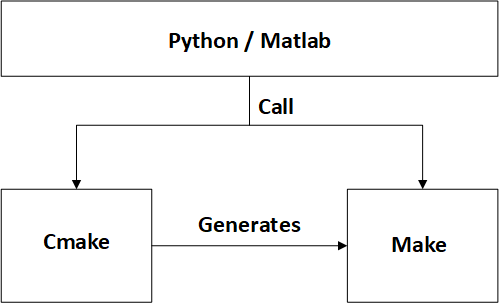
\includegraphics[width=0.5\textwidth]{build_system}
	\caption{Build system}
	\label{fig:build system}
\end{figure}
In order to easily simulate the controller from Python, the Python code must be able to call the functions inside the compile library. This is accomplished using the Ctypes library, Which allows Python scripts to directly call C functions.(If the dynamic library has the necessary properties)

Matlab can also call directly into a dynamic library, this is accomplished through the callib function in Matlab. The same compiled shared library can be used for either Matlab or Python.

\subsection{How to use it with an embedded system}
After enough simulations have been executed, and the control parameters are found. It is advised to remove the generated code. Called the bootstrapper with the simulation tools disabled, and generate the code again. This time no build tools will be inside the code, and the user cannot simulate this controller from Python or Matlab.

The include folder contains the header file for the controller, as the only header file relevant to the user. Which contains a initialize function, a function to set the weight of the obstacles, a function to get the optimal input given the current state and a destroy function. The initialize function shall be called at the startup of the controller. And to destroy function should be called when stopping the controller.

\begin{lstlisting}[caption={Header file of the controller},label={lst:Header file of the controller}]
int nmpc_init(void);
int nmpc_cleanup(void);
int npmc_solve( const real_t* current_state,
	const real_t* state_reference,
	const real_t* input_reference,
	real_t* optimal_inputs);
int nmpc_get_last_full_solution(real_t* output);

real_t nmpc_get_weight_obstacles(int index_obstacle);
int nmpc_set_weight_obstacles(int index_obstacle,real_t weight);
int nmpc_set_buffer_solution(real_t value, int index); 
\end{lstlisting}
\chapter{Simulation}
This chapter discusses some simulation results, using a simple mathematical model to create a controller. First the mathematical model is discussed, after that the simulation results are discussed and compared with the internal Matlab solvers.

\section{Model complexity}
The trailer model has a very low computational complexity, which makes it cheap to simulate with. The quad copter model, is a very complex model, that requires lots of computations for each simulation step. In this chapter it will become clear that PANOC is a very good with simple models, but a significantly slower with complex models compared to a interior point method.


\section{Trailer model}
The trailer model is illustrated in figure~\ref{fig:trailer model}, the left rectangle is the trailer and the right rectangle is the driver. The driver pulls the trailer forward. The driver is connect to the trailer via a single arm as illustrated in figure~\ref{fig:trailer model}. The control system can only change the speed in the Y and X axis. The goal of the control system is to get the trailer at a certain position and at a certain angle. Figure shows the trailer in a neutral position, so under an angle of 0 degrees.

\begin{figure}
	\centering
	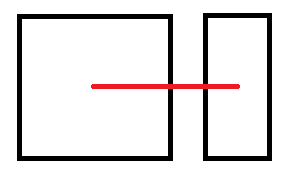
\includegraphics[width=0.5\textwidth]{trailer}
	\caption{Trailer model scheme}
	\label{fig:trailer model}
\end{figure}

The mathematical model of the trailer is represented in \eqref{eq:trailer model}, $u_x$ and $u_y$ are the inputs of the system and represent the speed in the Y and X direction. The angle is represented by $\theta$ , the distance between the driver and the trailer is represented by L. The position of the trailer is represented by $p_x$ and $p_y$.

\begin{equation}
	\begin{cases}
		\dot{p_x} = u_x + L sin \theta \cdot \dot{\theta} \\
		\dot{p_y} = u_y + L cos \theta \cdot \dot{\theta} \\
		\dot{\theta} = \frac{1}{L}(u_ycos \theta - u_x sin \theta)	
	\end{cases}
	\label{eq:trailer model}
\end{equation}

\section{A simple trailer example}
A simple way of measuring the performance of the library is to compared it to the alternatives. In the following simulation the nmpc-codegen library will be compared to, ForBes zerofrp2 the Matlab implementation of the PANOC algorithm. And to the internal Matlab function fmincon using either of the tree algorithms interior point,SQP and active set.

\subsection{General performance}
Several NMPC problems can be constructed and solved with nmpc-codegen. Figure~\ref{fig:demos} illustrates the problems used to benchmark nmpc-codegen, they all use the simple trailer model but have different obstacles. The time till convergence is measured, the average time is displayed in table~\ref{tbl:mean time till convergence} in the appendix. While the maximum and minimum time is displayed in the appendix: table~\ref{tbl:min time till convergence} and table~\ref{tbl:max time till convergence}.

The convergence time can be expresses relatively to the convergence time of the nmpc-codegen time as illustrated by \eqref{eq:definition relative time}. These results are displayed in table~\ref{tbl:mean relative time till convergence}. From table~\ref{tbl:mean relative time till convergence} it's clear that nmpc-codegen dominates by a significant margin.

\begin{equation}
	t_{relative} = \frac{t_{algorithm}}{t_{nmpc-codegen}}
	\label{eq:definition relative time}
\end{equation}

\subsection{In-dept analysis of performance}
The in-dept simulation contains four circular obstacles, the trailer will move from the lower left corner to the upper right corner. Each of the algorithms will calculate the optimal path up to the tolerance of $10^{-3}$. The input for one step is then applied to the system equation, and the next state is obtained. The same nmpc problem is solved using the new state as current state  and the new input is applied again.

The state of the trailer will is represented by arrows, the starting point of the arrow is the position of the trailer. The angle of the arrow represents the positional angle of the trailer. The amplitude of the arrow has no meaning.

Figure~\ref{fig:solution path trailer example} contains the results of the simulation. The PANOC algorithm calculated the lowest located path while all three of the fmincon algorithms opted for the upper located path. Both of these paths are valid solutions. It is immediately clear from figure~\ref{fig:timings trailer example} that the nmpc-codegen library is significantly faster. The other four algorithm's are about the same for the first 30 steps, after about 30 steps the ForBes zerofpr2 algorithm is faster then either of the tree fmincon algorithms.

The nmpc-codegen library uses a cautious L-BFGS update which improves the performance of the L-BFGS. This is clear from figure~\ref{fig:iterations trailer example} where not the time to convergence but iterations till convergence are illustrated. The nmpc-codegen clearly needs less iterations than  Forbes zerofpr2. As the simulation progresses, less and less iterations are needed to calculate optimal solution. And the L-BFGS doesn't influence the convergence as much, so the two algorithms have about the same amount iterations till convergence.
\begin{figure}[H]
	\centering
	\begin{subfigure}[b]{0.45\textwidth}
		\centering
		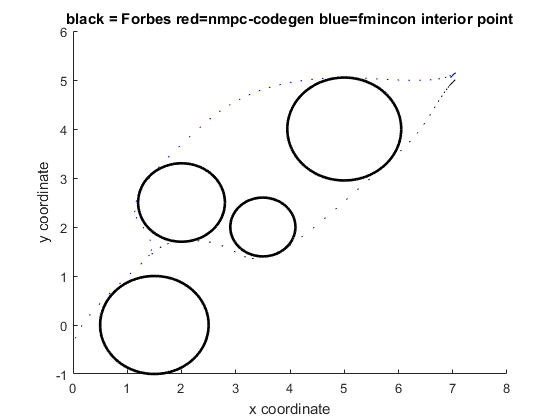
\includegraphics[width=1.2\textwidth]{compare_libs/path}
		\caption{path}
		\label{fig:solution path trailer example}
	\end{subfigure}
	
	\begin{subfigure}[b]{0.45\textwidth}
		\centering
		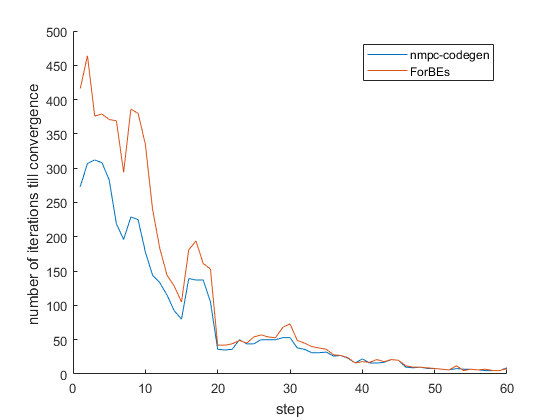
\includegraphics[width=1.2\textwidth]{compare_libs/iterations}
		\caption{iterations}
		\label{fig:iterations trailer example}
	\end{subfigure}
	\hfill
	\begin{subfigure}[b]{0.45\textwidth}
		\centering
		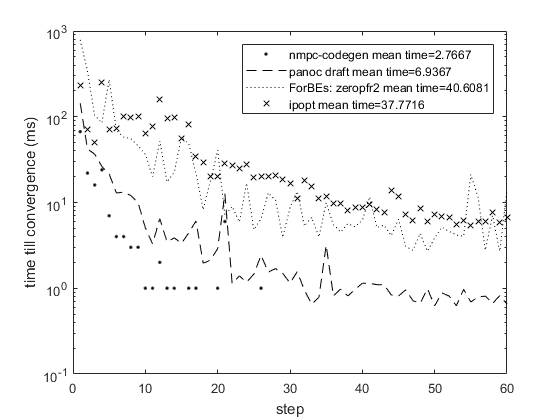
\includegraphics[width=1.2\textwidth]{compare_libs/timings}
		\caption{timings}
		\label{fig:timings trailer example}
	\end{subfigure}
	\caption{Simulation result trailer model}
\end{figure}

\section{Quadcopter model}
%TODO: reference source model !!!!!!!!!!!!!!!!!!
The invention of electronic control systems has proven to be especially useful when controlling quadcopters. Because of their complex behavior they are hard to control manually by a pilot. However quadcopters are popular among unmanned aerial vehicles but they are controlled by a fast digital/analog controller.

\subsection{Mathematical model}
The behavior of a quad copter is described by a set of nonlinear equations as illustrated in \eqref{eq:mathematical model quadcopter}.

\begin{table}[]
	\centering
	\caption{constants used in quadcopter model}
	\label{btl:quadcopter model constants}
	\begin{tabular}{|l|l|l|l|}
		\hline
		Parameter                               & Symbol   & Value             & Unit           \\ \hline
		Mass of the quadcopter                  & m        & 0.5               & kg             \\
		Radius of the quadcopter                & L        & 0.25              & m              \\
		Propeller lift coefficient              & k        & $3 \cdot 10^{-6}$ & $Ns^2$        \\
		Propeller drag coefficient              & b        & $1 \cdot 10^{-7}$ & N m $s^2$      \\
		Acceleration of gravity                 & g        & 9.81              & m/$s^2$        \\
		Air friction coefficient                & $k_d$    & 0.25              & kg/s           \\
		Quadcopter inertia about the $x^b$-axis & $I_{xx}$ & $5 \cdot 10^{-3}$ & kg $m^2$       \\
		Quadcopter inertia about the $y^b$-axis & $I_{yy}$ & $5 \cdot 10^{-3}$ & kg $m^2$       \\
		Quadcopter inertia about the $z^b$-axis & $I_{zz}$ & $1 \cdot 10^{-2}$ & kg $m^2$       \\ 
		Motor constant                          & $c_m$    & $1 \cdot 10^{4}$  & $v^{-2}s^{-2}$ \\
		\hline
	\end{tabular}
\end{table}

\begin{equation}
	\begin{aligned}
		\dot{x} &= v_x \\
		\dot{y} &= v_y \\
		\dot{z} &= v_z \\
		\dot{v_x} &= -\frac{k_d}{m}v_x + \frac{k \cdot c_m}{m}\Big(sin(\gamma)sin(\phi)+cos(\gamma)cos(\phi)sin(\theta)\Big)\Big(u_1 + u_2 + u_3 + u_4\Big) \\
		\dot{v_y} &= -\frac{k_d}{m}v_y + \frac{k \cdot c_m}{m}\Big(cos(\phi)sin(\gamma)sin(\theta)-cos(\gamma)sin(\phi)\Big)\Big(u_1 + u_2 + u_3 + u_4\Big) \\
		\dot{v_z} &= -\frac{k_d}{m}v_y -g + \frac{k \cdot c_m}{m}\Big(cos(\theta)cos(\phi)\Big)\Big(u_1 + u_2 + u_3 + u_4\Big) \\
		\dot{\phi} &= \omega_x + \omega_y\Big( sin(\phi)tan(\theta) \Big) + \omega_z \Big( cos(\phi) tan(\theta) \Big) \\
		\dot{\theta} &= \omega_y cos(\phi) - \omega_z sin(\phi) \\
		\dot{\gamma} &= \frac{sin(\phi)}{cos(\theta)}\omega_y + \frac{cos(\phi)}{cost(\theta)} \omega_z \\
		\dot{\omega_x} &= \frac{Lkc_m}{I_{xx}}\Big( u_1 - u_3 \Big) - \Big( \frac{I_{yy}-I_{zz}}{I_{xx}} \Big) \omega_y \omega_z\\
		\dot{\omega_y} &= \frac{Lkc_m}{I_{yy}}\Big( u_2 - u_4 \Big) - \Big( \frac{I_{zz}-I_{xx}}{I_{yy}} \Big) \omega_x \omega_z\\
		\dot{\omega_z} &= \frac{bc_m}{I_{zz}}\Big( u_1 - u_2 + u_3 - u_4 \Big) - \Big( \frac{I_{xx}-I_{yy}}{I_{zz}} \Big) \omega_x \omega_y\\
	\end{aligned}
	\label{eq:mathematical model quadcopter}
\end{equation}

\subsection{Simulation results}
Figure~\ref{fig:Simulation results with quadcopter} contains a simple simulation with the quad copter model, the path is displayed in figure~\ref{fig:solution path trailer quad}. The two sphere shaped obstacles, and the quad copter is moving from the star symbol to the circle. The time to convergence of each step of the simulation, is displayed in figure~\ref{fig:timings trailer quad}.

As mentioned at the start of this chapter, the quad copter model computational expensive model. This means that the computational cost of solving a system, is more in line with the computational cost of simulating one step of the system. 

A interior point method, must solve a system at each step of the algorithm. The interior method used from ipopt solves the system directly with a computational cost of about $\mathcal{O}(n^3)$ . While PANOC only has to cope additional cost of about $\mathcal{O}(Ln)$ with L as the buffer size.  because the L-BFGS algorithm only uses inner products and vector additions.

This means that the difference between PANOC and ipopt is rather small with the quad copter model. Which is clearly visible, in figure~\ref{fig:timings trailer quad}, where the ipopt line is very near the ipopt line.
\begin{figure}[H]
	\centering
	\begin{subfigure}[b]{0.45\textwidth}
		\centering
		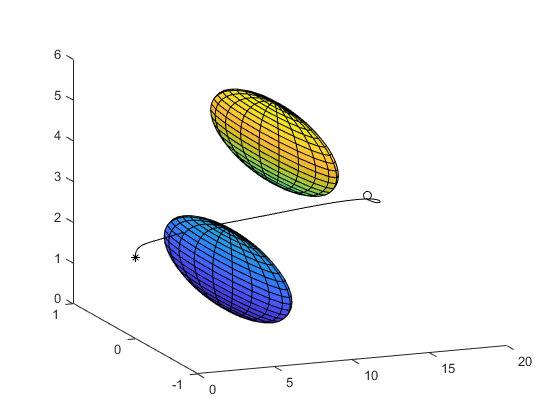
\includegraphics[width=1.2\textwidth]{compare_libs/path_quad}
		\caption{path}
		\label{fig:solution path trailer quad}
	\end{subfigure}
	\hfill
	\begin{subfigure}[b]{0.45\textwidth}
		\centering
		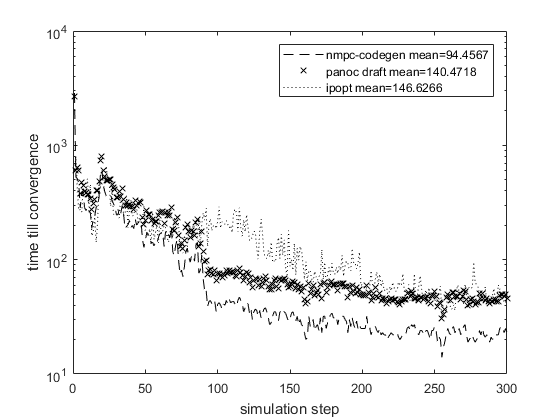
\includegraphics[width=1.2\textwidth]{compare_libs/timings_quad}
		\caption{timings}
		\label{fig:timings trailer quad}
	\end{subfigure}
	\caption{Simulation results with quadcopter}
	\label{fig:Simulation results with quadcopter}
\end{figure}

\section{Influence of noise}
Until now all simulations were executed without any kind of noise. However in reality there is always some kind of state noise. So is essential to study how PANOC handles state noise.

The white noise has a maximum amplitude of 0.1 on the x state and the y state. It has a amplitude of 0.05 on the angle $\theta$. The double noise simply doubles the maximum amplitude of the noise. This way the influence of the size of the noise can be studied.

Figure~\ref{fig:Noise simulations with the trailer model} contains the simulation results using PANOC or ipopt as solver. Going from no state noise to a bit of state noise makes a significant difference when solving with PANOC. The interior point method from ipopt, thus take longer to converge when noise is added. However it is less proportional towards the noise, as the interior point method here uses a direct method to solve the system.

\begin{figure}[H]
	\centering
	\begin{subfigure}[b]{0.45\textwidth}
		\centering
		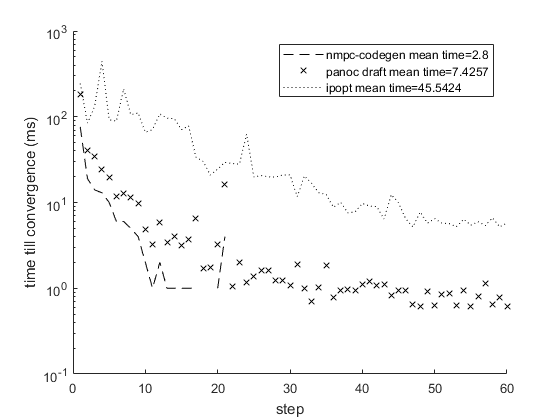
\includegraphics[width=1.2\textwidth]{compare_libs/trailer_without_noise}
		\caption{without noise}
		\label{fig:timings trailer without noise}
	\end{subfigure}
	\hfill
	\begin{subfigure}[b]{0.45\textwidth}
		\centering
		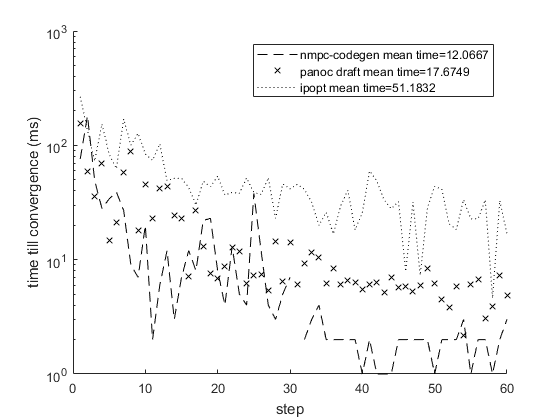
\includegraphics[width=1.2\textwidth]{compare_libs/trailer_with_noise}
		\caption{with noise}
		\label{fig:timings trailer with noise}
	\end{subfigure}
	\begin{subfigure}[b]{0.45\textwidth}
		\centering
		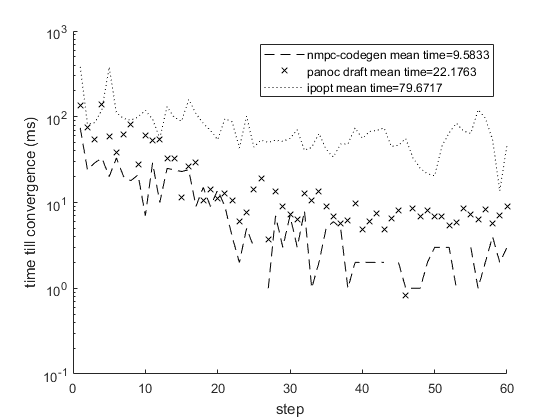
\includegraphics[width=1.2\textwidth]{compare_libs/trailer_with_double_noise}
		\caption{with double noise}
		\label{fig:timings trailer with double noise}
	\end{subfigure}
	\hfill
	\begin{subfigure}[b]{0.45\textwidth}
		\centering
		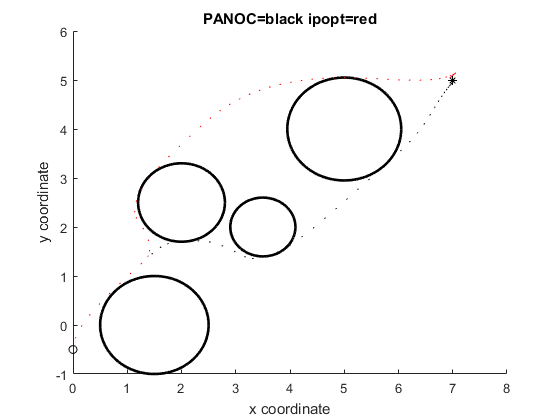
\includegraphics[width=1.2\textwidth]{compare_libs/path_without_noise}
		\caption{path without noise}
		\label{fig:path noise simulations}
	\end{subfigure}
	\caption{Noise simulations with the trailer model}
	\label{fig:Noise simulations with the trailer model}
\end{figure}

\begin{table}[H]
	\centering
	\begin{tabular}{|l|c|c|c|c|}
		\hline
		&\textbf{no noise}&\textbf{with noise}&\textbf{double noise}\\\hline
		\textbf{nmpc-codegen}&3 ms&12 ms&10 ms \\\hline
		\textbf{draft PANOC}&8 ms&18 ms&22 ms \\\hline
		\textbf{OPTI:ipopt}&45 ms&51 ms&80 ms \\\hline
	\end{tabular}
	\caption{average till convergence in milliseconds}
	\label{tbl:average till convergence noise}
\end{table}

\section{Problem with local minimum}
One problem with the approach discussed in this chapter, it's visible in the third demo. The results of the third demo are illustrated in figure~\ref{fig:demo: local minimum problem}, the trailer drives through the obstacle which is obviously impossible in reality. In reality the trailer will simply crash into the obstacle, and get stuck. Of course it is possible to increase the weight on the obstacle, this will make the problem harder. As the condition will get worse, and the solution will be about the same. The trainer will get stuck against the obstacle.

\begin{figure}[H]
	\centering
	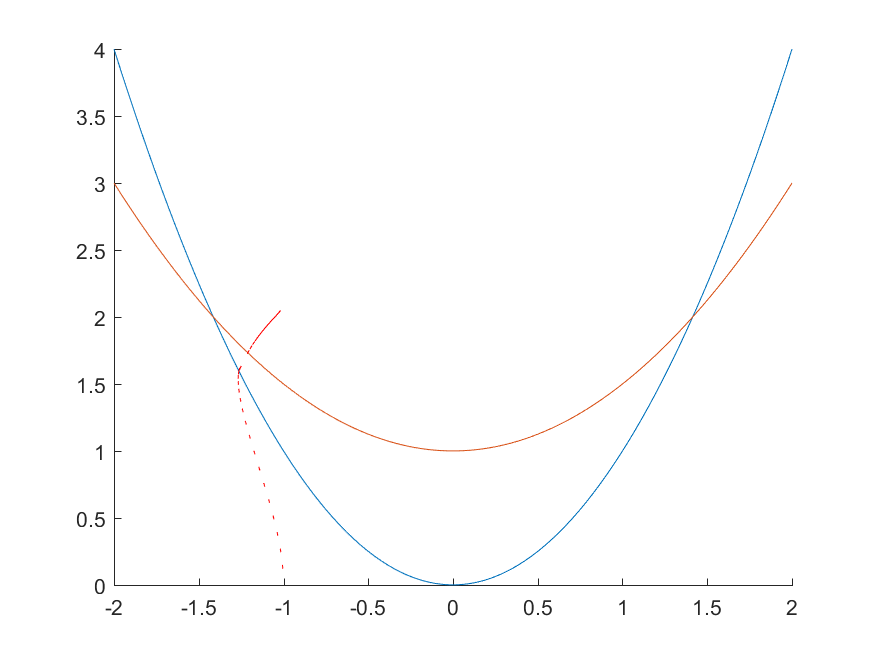
\includegraphics[width=0.5\textwidth]{demos/demo3}
	\caption{Local minimum problem}
	\label{fig:demo: local minimum problem}
\end{figure}

\section{Conclusion}

The simulations clearly indicate that a great speed up his gained by implementing the PANOC algorithm in C. As the algorithm doesn't require a lot of memory it can be run efficiently on small embedded devices. The control engineer can design and test the performance of the algorithm in either Matlab or Python.
\chapter{Code analysis of PANOC}
The speed of the Matlab or Python code is not very relevant as it only generates source files, its performance is not linked to the controller's performance. The generated C code on the other hand should have a good performance, as it determines the performance of the actual controller.

It is important to measure where most of the execution time is spent inside the algorithm. As this will indicate where to optimize the code. One way to measure this is by using profilers, in this chapter the results of the GNU profiler and the Intel profiler will be studied.

In order to get consistent results which profilers, the code execution must be long enough. And the problem that is being solved, must be sufficiently hard. So it will not converge in only a few steps. Because if it does converge in just a few steps, the cost function and its gradient will be the dominant cost factor. They will take over 90\% of the execution time, and as they are generated by Casadi, there's not much that can be done.

However if the problem is hard enough to solve, the quasi Newton method will be relevant. The buffer will be filled up, and the actual implementation of the algorithm will influence the performance significantly.

The problems used this chapter is displayed in Figure~\ref{fig:solution nmpc problem analysis}. In order to get consistent results, the execution time must be sufficiently long. This is why the same simulations is executed 500 times sequentially while the profiler runs.

\begin{figure}[H]
	\centering
	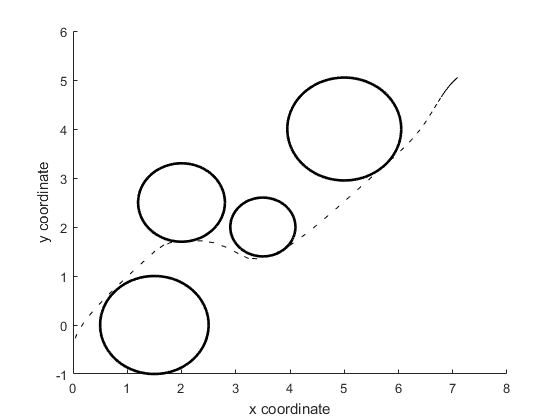
\includegraphics[width=0.5\textwidth]{intel_analysis/solution}
	\caption{Solution nmpc problem analysis}
	\label{fig:solution nmpc problem analysis}
\end{figure}

\section{Intel Profiler}
The first profiler that will be discussed is Intel's Vtune Amplifier. In order to make the profiling easier, only one cost/gradient function will be used for both the cost function and its gradient. This means that evaluating the cost function, also means evaluating the gradient.

\subsection{Hot spot analysis}
The Intel profiler contains a hotspot analysis, which finds the functions that take most time when executing the simulation. The results are displayed in Figure~\ref{fig:hotspot no mkl}.  It's quite clear from these results that the inner product and vector additions are two dominant costs inside the algorithm.

The most dominant cost is the cost function and its gradient, as this function is generated by the casadi library. There's nothing that can be done about it's performance. The PANOC algorithm is implemented in a way that the gradient/cost function is never evaluated twice at the same place.

The inner product and vector additions can be implemented using Intel's MKL math library. These routines are fine-tuned BLAS routines and are one of the fastest on the market. Replacing inner products and vector additions with these routines however does not significantly change the performance of the algorithm (results in firgure~\ref{fig:hotspot with mkl}), as the vectors used in this problem are too small to see a visible change. The BLAS functions just become the dominant cost now.

It is true that the aim of the nmpc-codegen library is to provide controller software for embedded devices. And embedded devices will most likely not have BLAS routines. Nevertheless this proves that putting a lot of time in optimizing the linear algebra routines might not always be very productive. The question is, how can the dependency on inner products and vector additions be reduced? The Intel profiler provides a function called bottom-up analysis. Bottom-up visualizes, who is calling all these inner products and vector additions.

%The trailer model uses sines and cosines, these are also expensive operations. More on the sine and cosines later on.
\begin{figure}[H]
	\centering
	\begin{subfigure}[b]{0.45\textwidth}
		\centering
		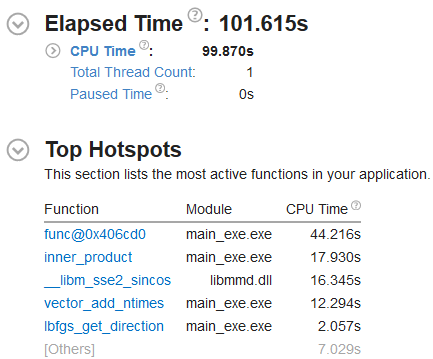
\includegraphics[width=1.2\textwidth]{intel_analysis/no_mkl}
		\caption{no mkl}
		\label{fig:hotspot no mkl}
	\end{subfigure}
	\hfill
	\begin{subfigure}[b]{0.45\textwidth}
		\centering
		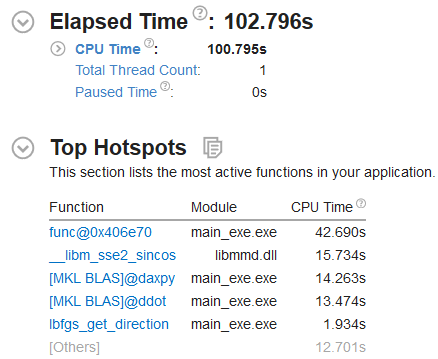
\includegraphics[width=1.2\textwidth]{intel_analysis/with_mkl}
		\caption{with mkl}
		\label{fig:hotspot with mkl}
	\end{subfigure}
	\caption{Hot spot analysis with Intel Vtune Amplifier 2018}
\end{figure}

Figure~\ref{fig:bottom-up analysis} provides a high-level view of the bottom-up analysis, Figure~\ref{fig:detailed bottom-up analysis} provides a detailed view of the bottom-up analysis. From the detailed view it is clear that most of the inner product and vector addition function calls are coming from the L-BFGS algorithm. This underlines the importance of choosing the right buffer size for the quasi Newton method. To further illustrate this, Figure~\ref{fig:Simulations with different buffer sizes} contains the simulation results for different buffer sizes.

\begin{figure}[H]
	\centering
	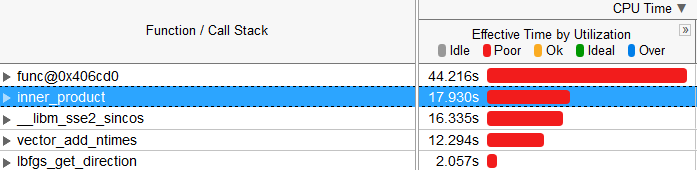
\includegraphics[width=0.7\textwidth]{intel_analysis/bottum_up}
	\caption{Bottom-up analysis}
	\label{fig:bottom-up analysis}
\end{figure}

\begin{figure}[H]
	\centering
	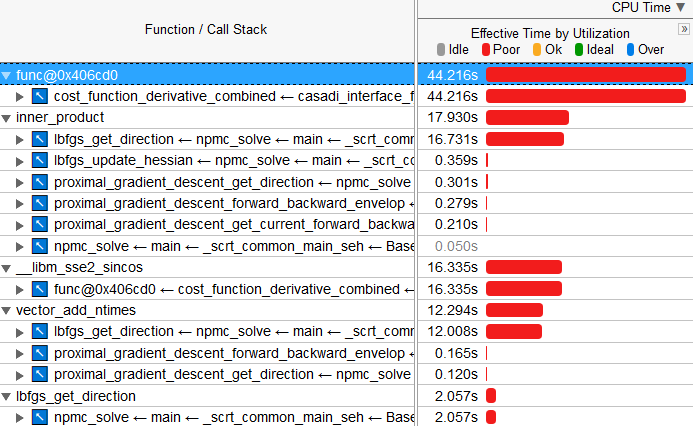
\includegraphics[width=0.7\textwidth]{intel_analysis/bottum_up_detailed}
	\caption{Detailed bottom-up analysis}
	\label{fig:detailed bottom-up analysis}
\end{figure}

The number of iterations till convergence is illustrated in Figure~\ref{fig:Simulations with different buffer sizes}, if no L-BFGS is used, the algorithm clearly needs significantly more iterations. However if the L-BFGS method is used it will decrease the amount iterations till convergence. The buffer size can be quiet small, as it doesn't seem to improve the performance when the size is greater then 10. This is visible from Figure~\ref{fig:different lbfgs buffer iterations till convergence},  where it is clear that a buffer size of 2, 7 or 200 can result in about the same convergence time.

The bigger the size of the L-BFGS buffer the more inner products and vector additions are required in each step. It is imperative to not only take a large enough buffer, but also not take it too large as this can significantly impact the performance.

\begin{figure}[H]
	\centering
	\begin{subfigure}[b]{0.45\textwidth}
		\centering
		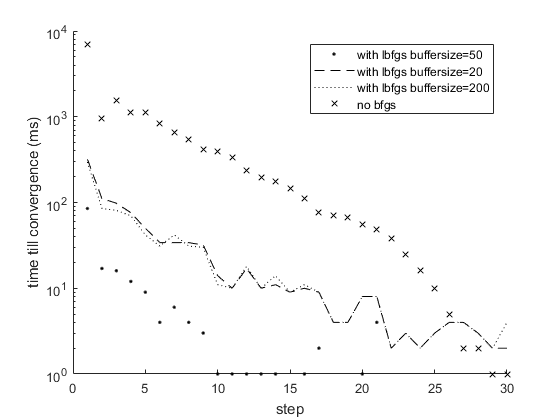
\includegraphics[width=1.2\textwidth]{compare_lbfgs_size/time_till_convergence}
		\caption{different L-BFGS buffer time till convergence}
		\label{fig:different lbfgs buffer time till convergence}
	\end{subfigure}
	\hfill
	\begin{subfigure}[b]{0.45\textwidth}
		\centering
		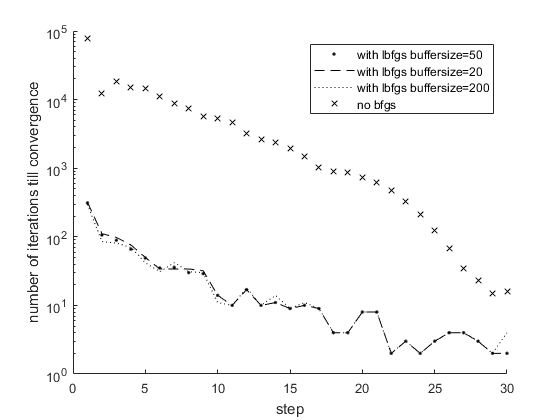
\includegraphics[width=1.2\textwidth]{compare_lbfgs_size/number_of_iterations}
		\caption{different L-BFGS buffer iterations till convergence}
		\label{fig:different lbfgs buffer iterations till convergence}
	\end{subfigure}
	\caption{Simulations with different buffer sizes}
	\label{fig:Simulations with different buffer sizes}
\end{figure}

The opposite of a bottum-up  analysis is a top down analysis, which determines how  much time the  function spends inside the functions it calls. The results of this analysis is illustrated in Figure~\ref{fig:no mkl top down}. Figure~\ref{fig:no mkl top down} indicates that about one third of the execution time is spend calculating the direction of the quasi Newton method. The two most dominant costs when calculating this direction are the inner products and the vector addition.

The rest of the time is mostly spent calculating the gradient and cost function. The proximal gradient method, is not so dependent upon inner products and vector additions. This is also visible in the caller callee analysis displayed in table~\ref{tbl:Caller Callee analysis}, about 61\% of the time is spent calculating the gradient. If the problem is easier to solve, or the buffer is smaller, then the cost of the gradient is even more dominant. And can easily go up to 80\% or 90\%. This is why a hard problem was used when profiling the algorithm. If an easy problem was used, then the results become irrelevant as the relative costs of the gradient will make everything else irrelevant.

\begin{figure}[H]
	\centering
	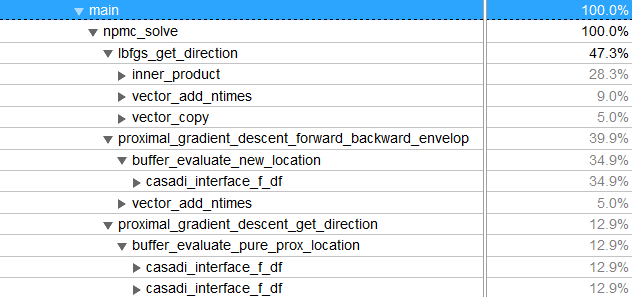
\includegraphics[width=0.7\textwidth]{intel_analysis/no_mkl_topdown}
	\caption{Top down analysis}
	\label{fig:no mkl top down}
\end{figure}

\begin{center}
	\begin{tabular}{| l | c |}
		\hline
		Function&CPU Time: Total (\%) \\
		\hline
		casadi\_interface\_f\_df&61.2087\% \\
		proximal\_gradient\_descent\_forward\_backward\_envelop&36.9998\% \\
		buffer\_evaluate\_new\_location&34.7744\% \\
		lbfgs\_get\_direction&31.6374\% \\
		proximal\_gradient\_descent\_get\_direction&27.168\% \\
		buffer\_evaluate\_pure\_prox\_location&25.6641\% \\
		inner\_product&17.9297\% \\
		\_\_libm\_sse2\_sincos&16.335\% \\
		vector\_add\_ntimes&12.2935\% \\
		lbfgs\_update\_Hessian&1.74661\% \\
		\hline
	\end{tabular}
	\captionof{table}{Caller/Callee analysis}
	\label{tbl:Caller Callee analysis}
\end{center}

\section{Valgrind callgrind}
The Intel profiler combined with the Visual Studio shell is incredibly easy to use and very productive. However it is a proprietary piece of software, and a rather expensive one. The Intel profiler uses the Intel compiler, which often makes for better results with numerical computations then using the GNU compiler. So it is worth while to investigate the results with the GNU compiler.

One way of profiling with the GNU compiler is using valgrind with the option callgrind. Figure~\ref{fig:callgrid} displays the results of callgrind in a drawing. The relative execution time of the gradient is only 53\% instead of 61\% with the Intel compiler. It confirms the results obtained with the Intel profiler, as the inner products and vector additions are even more dominant here.

\begin{figure}[H]
	\centering
	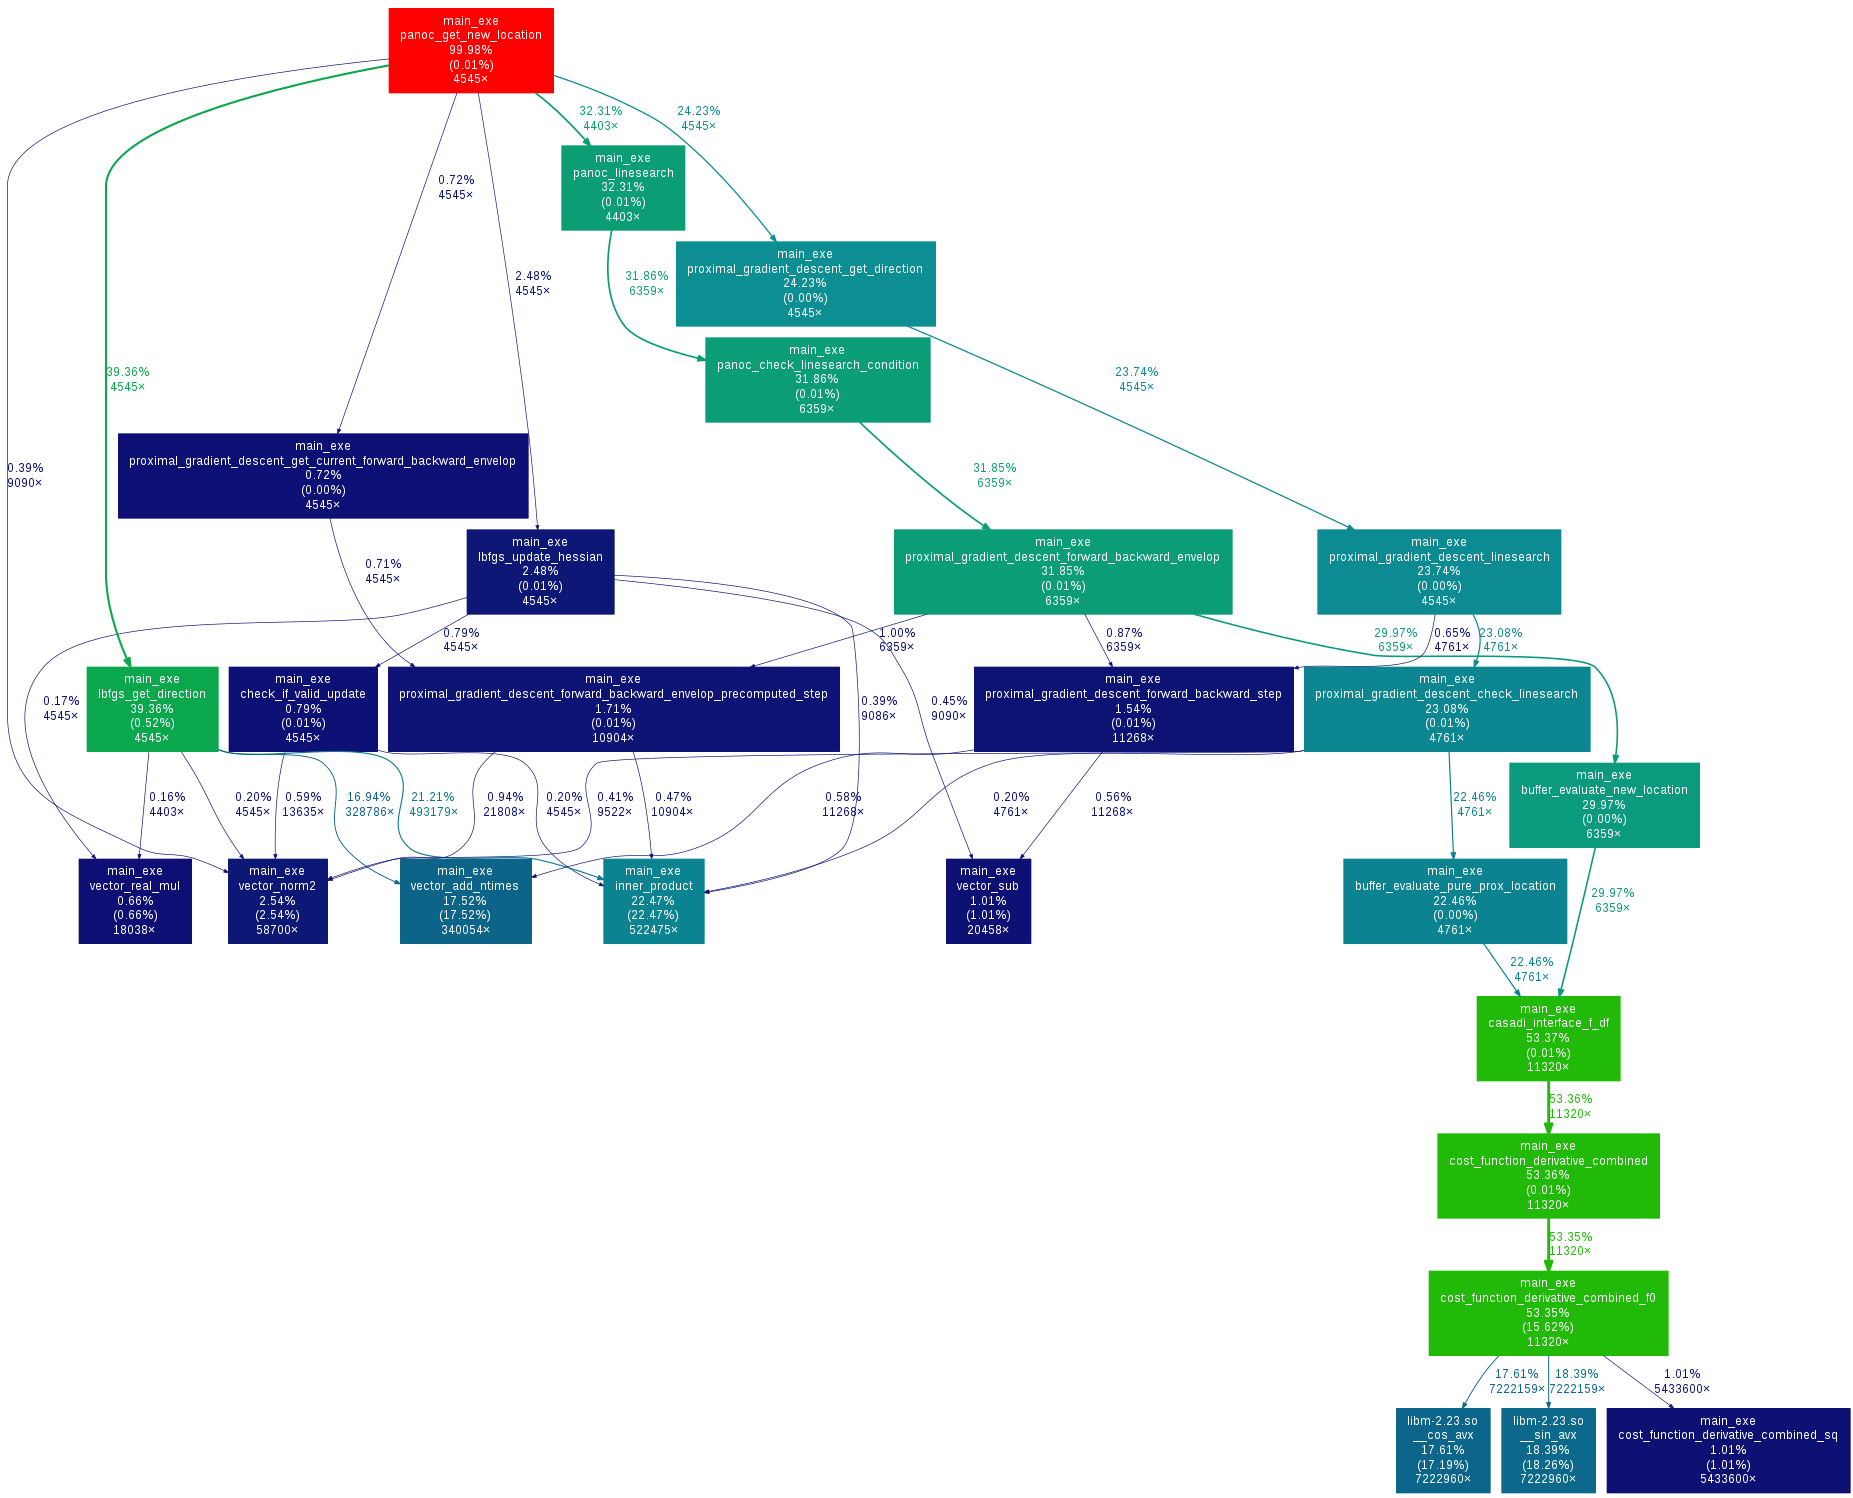
\includegraphics[width=1\textwidth]{callgrid/graph}
	\caption{Callgrid drawing}
	\label{fig:callgrid}
\end{figure}

\section{Conclusion}
The user should be careful when selecting the size of the buffer. If the buffer is too small the convergence will be slow. If the buffer is too large the quasi Newton method will require all lot more inner products and vector additions, which will significantly increase the time to convergence.

\chapter{The accelerated Lagrangian}

	\cite{Wright}
	
	\begin{equation}
		\Lagr_A(x,\lambda;\mu) \overset{def}{=} f(x) - \sum_{i \in \epsilon}\lambda_ic_i(x) + \mu \sum_{i \in \epsilon}c_i^2(x)
	\end{equation}

	\section{Optimality conditions}
		\begin{equation}
			\nabla_x \Lagr_A(x_k,\lambda_k;\mu_k) = \nabla f(x_k) - \sum_{i \in \epsilon} [\lambda_i^k - 2\mu_k c_i(x_k)] \nabla c_i(x_k)
		\end{equation}
		
		\begin{equation}
			\bar{\lambda_i} = \lambda_i - 2\mu_k c_i(x_k)
		\end{equation}
		
		
\chapter{Conclusion}
\label{cha:conclusion}

\section{Nmpc-codegen library}
The controller code generation and simulation is available in both Python and Matlab, which are computer languages with a fast learning curve. It is very straightforward for a control engineer to design and test a controller, without knowing anything about low level programming.

The generated controller, has a simple interface that requires nearly no control theory knowledge. So that the user of the generated C library doesn't necessarily has to be a control engineer but could be an embedded software engineer. Who has no idea how a MPC controller works, but knows how embedded systems work.

However as the MPC problem becomes more complex. The algorithm can get stuck on a local minimums, which might not be a viable solution. It might violate the constraint by a too large margin. This can partially be avoided by properly tuning the weights of the constraints. 

This weight tuning is rather hard, as increasing the weights worsens the condition of the problem. So the controller designer often ends up with an impossible choice. The last chapter partially solves this by using a Lagrangian. It is easier to tune the parameters and it improves the performance of the controller. 

\section{Future work}
The PANOC algorithm does not require advanced algebra operations such as solving a system. Only simple vector additions and inner product are required. So it's straightforward to implement PANOC with flip-flops and adders. The only hard part is the cost function and it's gradient, as Casadi does not support VHDL or Verilog at this time.

\section{Industrial applications}
Embedded model predictive control is used in a wide variety of domains, here are a few examples:
\begin{itemize}
	\item Unmanned Aerial vehicles (UAV's)
	\item Self driving robots
	\item Anti-lock brakes cars
	\item Adaptive cruise control cars
	\item Robotics
\end{itemize}

%%% Local Variables: 
%%% mode: latex
%%% TeX-master: "thesis"
%%% End: 

% If you have appendices:
\appendixpage*          % if wanted
\appendix
\chapter{Abstract Dutch}
Moderne controle systemen maken vaak gebruik van "model predictive control" algoritmes. Wanneer lineaire modellen gebruikt worden, moet een stelsel van lineaire vergelijkingen worden opgelost. De algoritmes voor het oplossen van een stelsel van lineaire vergelijkingen zijn uitgebreid onderzocht en ge\"{i}mplementeerd. 

Wanneer een niet-lineaire model wordt gebruikt, moet een niet-lineaire stelsel opgelost worden. Dit stelsel kan worden opgelost met iteratieve algoritmes zoals "interior point" of SQP algoritmes. Deze algoritmes gebruiken veel geheugen, wat ze vaak ondergeschikt maken voor embedded toepassingen. Het "proximal gradient" algoritme gebruikt weinig geheugen maar heeft slechts sub lineaire convergentie. Dit is waar het PANOC algoritme interessant wordt, het kan namelijk een niet lineaire stelsel oplossen met veel minder geheugen dan een "interior point" algoritme. Maar heeft wel super lineaire convergentie. 

Het doel van deze masterproef is een raamwerk te implementeren die een niet-lineaire MPC controller genereert in C. De controller maakt gebruik van het PANOC algoritme voor het oplossen van het niet lineaire stelsel. De code is specifiek gericht aan embedded toestellen, waardoor PANOC een uitstekende keuze is. De gebruiker van de software wordt verondersteld alleen controletheorie te kennen, en hoeft niets over PANOC algoritme noch embedded software te kennen.

De implementatie is gerealiseerd in Matlab en Python, aangezien dit de twee dominerende talen zijn bij computer simulaties van controlesystemen. Er wordt geen gebruik gemaakt van externe bibliotheken om de C code te genereren. Het PANOC is een convexe combinatie van het "proximal gradient" algoritme en L-BFGS. Er wordt gebruik gemaakt van het pakket Casadi om de gradi\"{e}nt te berekenen. Het is mogelijk om vanuit Matlab of Pyhton simulaties uit te voeren op de gegenereerde C code. Zo kunnen de nodige controle parameters afgesteld worden vanuit Matlab of Python.

De gegenereerde C code is getest met de GNU C compiler, Clang LLVM compiler, Microsoft C compiler en de Intel C compiler onder de ANSI C89 standaard. Er worden geen externe C bibliotheken gebruikt zodat de code eenvoudig kan gecompileerd worden voor verschillende platformen. Het enige noodzakelijke is een C compiler.

Vervolgens wordt aangetoond dat PANOC bij eenvoudige systemen sneller is dan "interior point" methodes, maar bij complexe systemen verliest het zijn snelheids voordeel. PANOC verbruikt wel altijd minder geheugen.

Tot slot is er recentelijk onderzoek ge\"{i}mplementeerd. Het toevoegen van voorwaarden op het controlesysteem kan namelijk leiden tot een slecht geconditioneerd probleem. De "augmented Lagrangian" methode bied hiervoor een oplossing. Door het probleem in verschillende stappen op te lossen kan er soms een beter resultaat bereikt worden.

\chapter{Mathematical definitions}
	\section{Box function}
	\label{appendix:box function}
		1 dimension:
		\begin{equation}
			\boxfunction_{1D}(u) =
			\begin{cases}
				 1 & u \in [-U_b:U_b]\\
				 0 & \other
			\end{cases}
			\label{eq:box function 1 dimension}
		\end{equation}
		N dimensions:
		\begin{equation}
			\boxfunction(u) = \min\left[ \sum_{k=1}^ N \boxfunction_{1D}(u) \right]
			\label{eq:box function N dimensions}
		\end{equation}
	\section{Indicator Box function}
	\label{appendix:indicator box function}
		\begin{equation}
			I_{\boxfunction}(u)=
			\begin{cases}
				0 & u \in [-U_b:U_b]\\
				\inf & \other
			\end{cases}
		\end{equation}
		
		\begin{equation}
			\prox_{\gamma I_{\boxfunction}}(u)=
			\begin{cases}
				u & u \in [-U_b:U_b]\\
				-U_b & u \in [-\inf:-U_b)\\
				-U_b & u \in (U_b:\inf]\\
			\end{cases}
		\end{equation}
	\section{Conjugate of strongly convex function}
	\label{appendix:conjugate of strongly convex function}
		\begin{equation}
			f^*(x)= \underset{u \in dom(f)}{<y,x>-f(y)}
		\end{equation}
		
		If $\nabla f^*$ is Lipschitz and obeys \eqref{eq:appendix f lip}, then $f^*$ is well defined and differentiable. (assume dom(f) is convex and closed)
		\begin{equation}
			\nabla f^*(x) = y^* = \argmax <y,x> - f(y)
		\end{equation}
		
		\begin{equation}
			|| \nabla f^*(x) - \nabla f^*(y) ||_2 \leq \mu^{-1} ||x-y||_2
			\label{eq:appendix f lip}
		\end{equation}
		
\chapter{Proof FBE alternative equation}
\label{appendix:proof FBE alternate equation}
\begin{proof}
	$\varphi_{\gamma} =   f(x) + \underset{y}{\inf} \Big\{ \nabla f(x)^T(y-x) + g(y) + \frac{1}{2 \gamma} ||x-y||^2  \Big\} $
	\begin{align*}
	g^{\gamma} 	&=  \underset{y}{\inf} \big \{f(y)+\frac{1}{2 \cdot \gamma}||x-y||^2 \big \} \\
	\varphi_{\gamma} 
	&= f(x) - \frac{\gamma}{2}||\nabla f(x)||^2 + g^{\gamma} \big(x-\gamma \nabla f(x) \big) \\
	&= f(x) - \frac{\gamma}{2}||\nabla f(x)||^2 + g^{\gamma} \big(\bar{x} \big)\\
	g^{\gamma} (\bar{x})
	&=\underset{y}{\inf} \Big\{g(y)+\frac{1}{2 \gamma}||\bar{x}-y||^2 \Big\}	\\
	\bar{x}^T\bar{x}
	&=[x- \gamma \nabla f(x)]^T[x- \gamma \nabla f(x)] \\
	&= x^Tx -2x^T\nabla f(x) \gamma + \gamma^2 \nabla f(x)^T\nabla f(x)-2x^Ty \\
	&=-2x^Ty + 2\gamma \nabla f(x)^Ty \\
	\frac{1}{2 \gamma}||\bar{x}-y||^2
	&=\frac{1}{2 \gamma} \Big [ (\bar{x}-y)^T(\bar{x}-y) \Big]\\
	&=\frac{1}{2 \gamma} \Big [ x^Tx - 2 x^Ty + y^Ty \Big]\\
	& = \frac{1}{2 \gamma}[-2x^T\nabla f(x) \gamma  + 2\gamma \nabla f(x)^Ty + \gamma^2 \nabla f(x)^T\nabla f(x) +x^Tx -2x^Ty +y^Ty]\\
	&= \frac{1}{2 \gamma}[ 2\gamma \nabla f(x)^T(y-x) + \gamma^2||\nabla f(x)||^2 + ||x-y||^2] \\
	&=  \nabla f(x)^T(y-x) +\frac{\gamma}{2}||\nabla f(x)||^2 + \frac{1}{2 \gamma} ||x-y||^2 \\
	g^{\gamma} (\bar{x})
	&=\underset{y}{\inf} \Big\{g(y)+ \nabla f(x)^T(y-x) +\frac{\gamma}{2}||\nabla f(x)||^2 + \frac{1}{2 \gamma} ||x-y||^2  \Big\} \\
	&= \frac{\gamma}{2}||\nabla f(x)||^2 + \underset{y}{\inf} \Big\{g(y)+ \nabla f(x)^T(y-x) + \frac{1}{2 \gamma} ||x-y||^2  \Big\} \\
	\varphi_{\gamma} 
	&= f(x) - \frac{\gamma}{2}||\nabla f(x)||^2 + g^{\gamma} \big(\bar{x} \big)\\
	&= f(x) - \frac{\gamma}{2}||\nabla f(x)||^2 +  \frac{\gamma}{2}||\nabla f(x)||^2 + \underset{y}{\inf} \Big\{g(y)+ \nabla f(x)^T(y-x) + \frac{1}{2 \gamma} ||x-y||^2  \Big\}\\
	&=   f(x) + \underset{y}{\inf} \Big\{ \nabla f(x)^T(y-x) + g(y) + \frac{1}{2 \gamma} ||x-y||^2  \Big\} 
	\end{align*}
	\label{prf:FBE alterative expression}
\end{proof}

\chapter{Benchmarks with trailer model}
\label{appendix:paths trailer simulations}

\begin{figure}[H]
	\centering
	\begin{subfigure}[b]{0.40\textwidth}
		\centering
		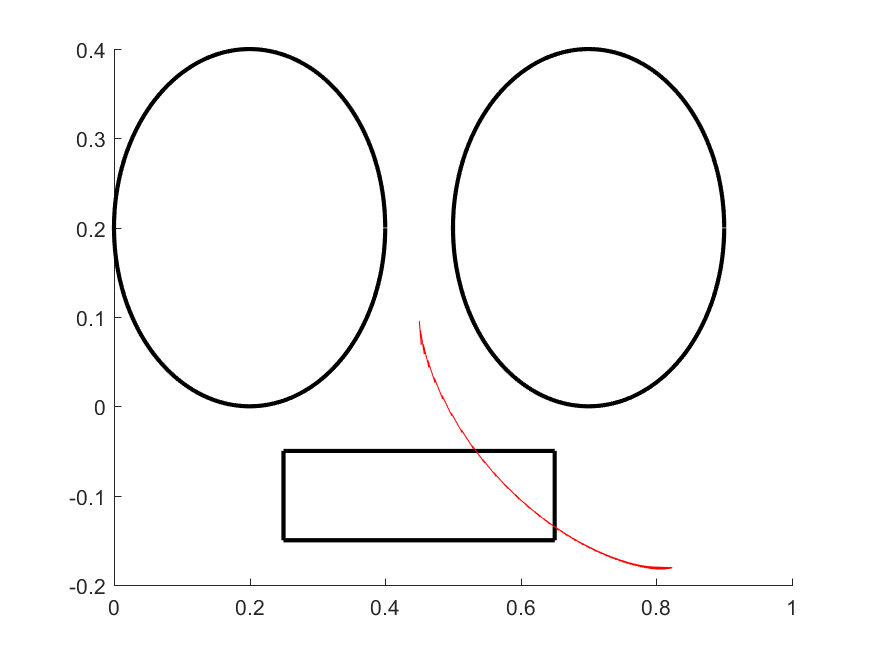
\includegraphics[width=1.2\textwidth]{demos/demo1}
		\caption{demo 1}
		\label{fig:demo 1}
	\end{subfigure}
	\hfill
	\begin{subfigure}[b]{0.40\textwidth}
		\centering
		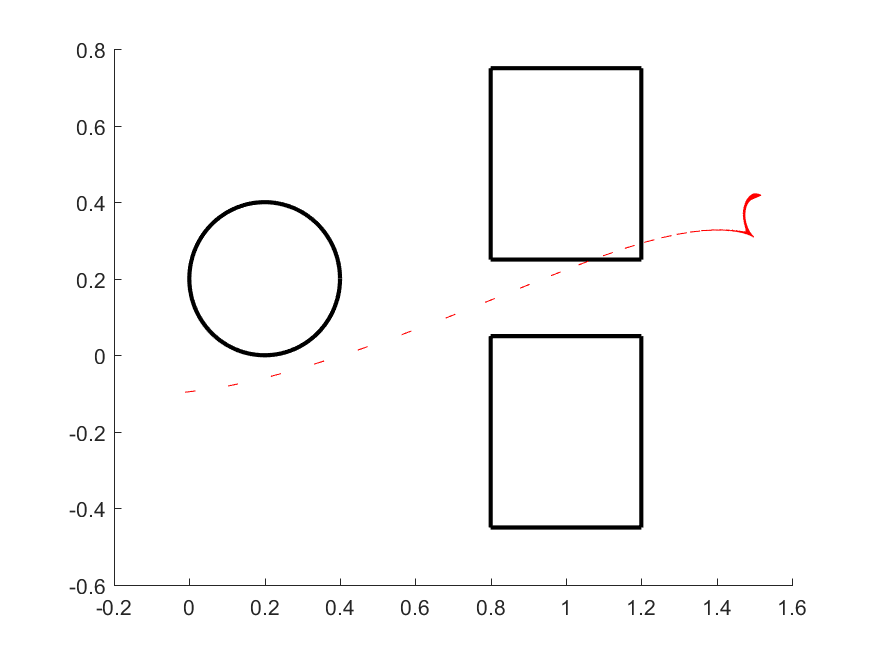
\includegraphics[width=1.2\textwidth]{demos/demo2}
		\caption{demo 2}
		\label{fig:demo 2}
	\end{subfigure}
	\begin{subfigure}[b]{0.40\textwidth}
		\centering
		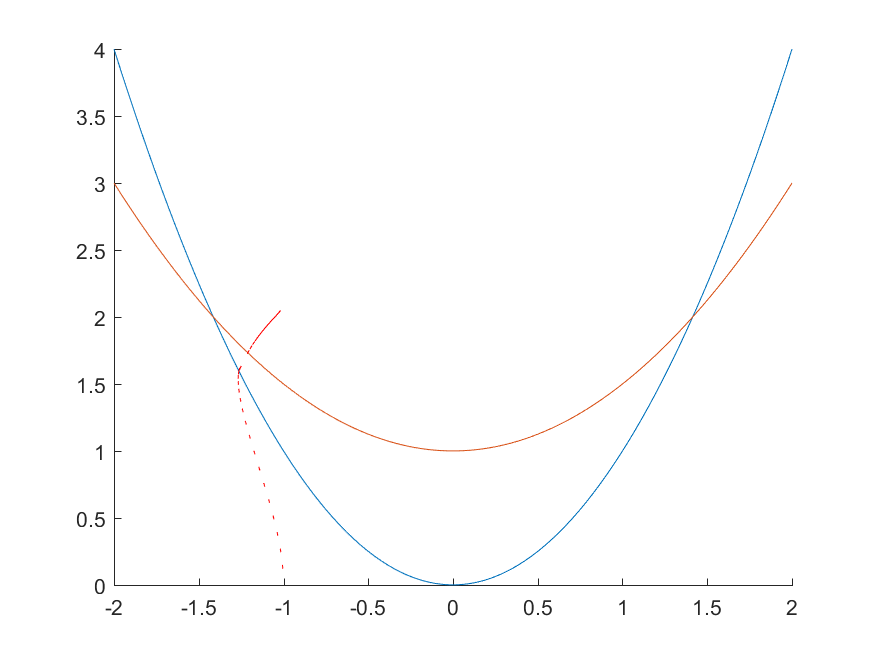
\includegraphics[width=1.2\textwidth]{demos/demo3}
		\caption{demo 3}
		\label{fig:demo 3}
	\end{subfigure}
	\hfill
	\begin{subfigure}[b]{0.40\textwidth}
		\centering
		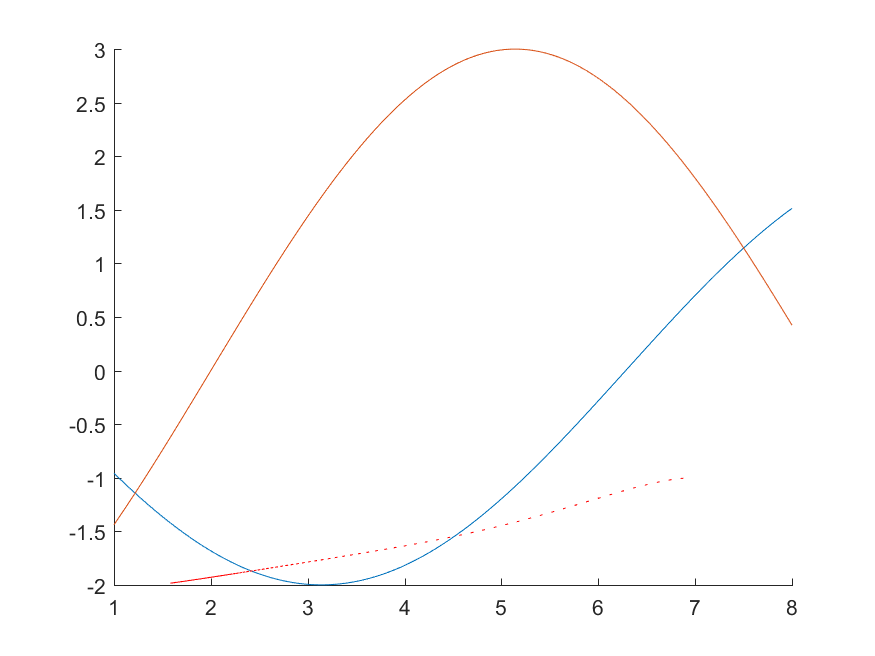
\includegraphics[width=1.2\textwidth]{demos/demo4}
		\caption{demo 4}
		\label{fig:demo 4}
	\end{subfigure}
	\caption{Path of demo's}
	\label{fig:demos}
\end{figure}
\begin{figure}[H]
	\centering
	\begin{subfigure}[b]{0.45\textwidth}
		\centering
		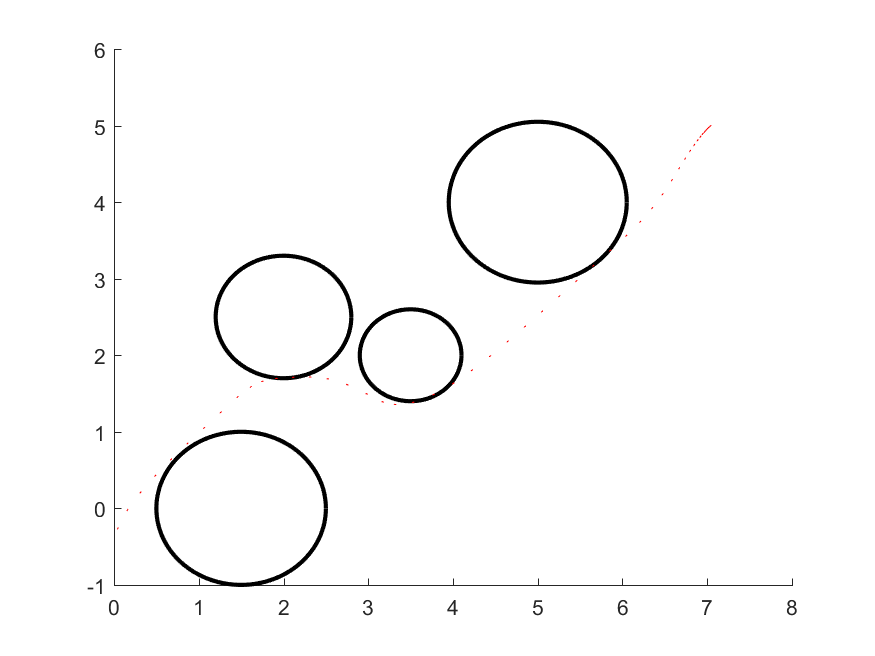
\includegraphics[width=1.2\textwidth]{demos/demo5}
		\caption{demo 5}
		\label{fig:demo 5}
	\end{subfigure}
\end{figure}

\section{Simulations without state noise}
\label{appendix:benchmarks trailer without noise}

\begin{table}[H]
	\centering
	\begin{tabular}{|l|c|c|c|c|}
		\hline
		&\textbf{demo5}&\textbf{demo2}&\textbf{demo3}\\\hline
		\textbf{nmpc-codegen (PANOC)}&9.00e-01&1.00e-01&4.10e-01\\\hline
		\textbf{ForBeS zerofrp2 (PANOC)}&2.99e+01&4.20e+00&5.56e+00\\\hline
		\textbf{PANOC draft}&5.73e+00&1.29e+00&2.00e+00\\\hline
		\textbf{fmincon:interior-point}&8.62e+01&2.31e+01&2.03e+01\\\hline
		\textbf{fmincon:sqp}&2.18e+01&1.15e+01&9.29e+00\\\hline
		\textbf{fmincon:active-set}&8.37e+01&2.36e+01&2.08e+01\\\hline
		\textbf{OPTI:ipopt}&3.79e+01&7.08e+00&8.21e+00\\\hline
	\end{tabular}
	\caption{mean time till convergence in milliseconds}
	\label{tbl:mean time till convergence}
\end{table}

\begin{table}[H]
	\centering
	\begin{tabular}{|l|c|c|c|c|}
		\hline
		&\textbf{demo5}&\textbf{demo2}&\textbf{demo3}\\\hline
		\textbf{nmpc-codegen (PANOC)}&100&100&100\\\hline
		\textbf{ForBeS zerofrp2 (PANOC)}&3323&4202&1357\\\hline
		\textbf{PANOC draft}&637&1289&489\\\hline
		\textbf{fmincon:interior-point}&9579&23107&4943\\\hline
		\textbf{fmincon:sqp}&2422&11469&2265\\\hline
		\textbf{fmincon:active-set}&9303&23578&5084\\\hline
		\textbf{OPTI:ipopt}&4213&7083&2003\\\hline
	\end{tabular}
	\caption{mean relative time till convergence in milliseconds}
	\label{tbl:mean relative time till convergence}
\end{table}

\begin{table}[H]
	\centering
	\begin{tabular}{|l|c|c|c|c|}
		\hline
		&\textbf{demo5}&\textbf{demo2}&\textbf{demo3}\\\hline
		\textbf{nmpc-codegen (PANOC)}&2.20e+01&8.00e+00&4.00e+01\\\hline
		\textbf{ForBeS zerofrp2 (PANOC)}&7.95e+02&1.25e+02&3.06e+02\\\hline
		\textbf{PANOC draft}&1.12e+02&3.66e+01&1.30e+02\\\hline
		\textbf{fmincon:interior-point}&1.55e+03&2.29e+02&2.95e+02\\\hline
		\textbf{fmincon:sqp}&1.01e+02&8.83e+01&1.10e+02\\\hline
		\textbf{fmincon:active-set}&7.83e+02&2.70e+02&2.45e+02\\\hline
		\textbf{OPTI:ipopt}&2.73e+02&4.65e+01&7.65e+01\\\hline
	\end{tabular}
	\caption{max time till convergence in milliseconds}
	\label{tbl:max time till convergence}
\end{table}

\begin{table}[H]
	\centering
	\begin{tabular}{|l|	c|c|c|c|}
		\hline
		&\textbf{demo5}&\textbf{demo2}&\textbf{demo3}\\\hline
		\textbf{nmpc-codegen (PANOC)}&0.00e+00&0.00e+00&0.00e+00\\\hline
		\textbf{ForBeS zerofrp2 (PANOC)}&2.11e+00&2.03e+00&2.01e+00\\\hline
		\textbf{PANOC draft}&5.16e-01&5.26e-01&5.16e-01\\\hline
		\textbf{fmincon:interior-point}&8.95e+00&8.35e+00&7.57e+00\\\hline
		\textbf{fmincon:sqp}&6.37e+00&6.58e+00&6.02e+00\\\hline
		\textbf{fmincon:active-set}&1.82e+01&1.63e+01&1.57e+01\\\hline
		\textbf{OPTI:ipopt}&5.03e+00&4.45e+00&4.37e+00\\\hline
	\end{tabular}
	\caption{min time till convergence in milliseconds}
	\label{tbl:min time till convergence}
\end{table}


\section{Simulations with state noise}
\label{appendix:benchmarks trailer with noise}

\begin{table}[H]
	\centering
	\begin{tabular}{|l|c|c|c|c|}
		\hline
		&\textbf{demo5}&\textbf{demo2}&\textbf{demo3}\\\hline
		\textbf{nmpc-codegen (PANOC)}&5.82e+00&4.20e-01&2.20e-01\\\hline
		\textbf{ForBeS zerofrp2 (PANOC)}&8.69e+01&1.19e+01&9.64e+00\\\hline
		\textbf{PANOC draft}&2.77e+01&4.54e+00&3.24e+00\\\hline
		\textbf{fmincon:interior-point}&3.17e+02&1.01e+02&8.15e+01\\\hline
		\textbf{fmincon:sqp}&9.07e+01&4.77e+01&3.93e+01\\\hline
		\textbf{fmincon:active-set}&2.29e+02&7.50e+01&6.46e+01\\\hline
		\textbf{OPTI:ipopt}&9.52e+01&1.41e+01&1.09e+01\\\hline
	\end{tabular}
	\caption{mean time till convergence in milliseconds}
	\label{tbl:mean time till convergence with noise}
\end{table}

\begin{table}[H]
	\centering
	\begin{tabular}{|l|c|c|c|c|}
		\hline
		&\textbf{demo5}&\textbf{demo2}&\textbf{demo3}\\\hline
		\textbf{nmpc-codegen (PANOC)}&100&100&100\\\hline
		\textbf{ForBeS zerofrp2 (PANOC)}&1494&2839&4383\\\hline
		\textbf{PANOC draft}&476&1080&1472\\\hline
		\textbf{fmincon:interior-point}&5453&24054&37058\\\hline
		\textbf{fmincon:sqp}&1560&11360&17870\\\hline
		\textbf{fmincon:active-set}&3937&17860&29378\\\hline
		\textbf{OPTI:ipopt}&1637&3362&4952\\\hline
	\end{tabular}
	\caption{mean relative time till convergence in milliseconds}
	\label{tbl:mean relative time till convergence with noise}
\end{table}

\begin{table}[H]
	\centering
	\begin{tabular}{|l|c|c|c|c|}
		\hline
		&\textbf{demo5}&\textbf{demo2}&\textbf{demo3}\\\hline
		\textbf{nmpc-codegen (PANOC)}&1.06e+02&1.30e+01&1.80e+01\\\hline
		\textbf{ForBeS zerofrp2 (PANOC)}&9.82e+02&2.23e+02&3.87e+01\\\hline
		\textbf{PANOC draft}&2.38e+02&7.07e+01&1.83e+01\\\hline
		\textbf{fmincon:interior-point}&2.45e+03&4.68e+02&3.40e+02\\\hline
		\textbf{fmincon:sqp}&4.22e+02&3.25e+02&4.18e+02\\\hline
		\textbf{fmincon:active-set}&1.13e+03&4.86e+02&5.69e+02\\\hline
		\textbf{OPTI:ipopt}&4.78e+02&9.21e+01&3.67e+01\\\hline
	\end{tabular}
	\caption{max time till convergence in milliseconds}
	\label{tbl:max time till convergence with noise}
\end{table}

\begin{table}[H]
	\centering
	\begin{tabular}{|l|	c|c|c|c|}
		\hline
		&\textbf{demo5}&\textbf{demo2}&\textbf{demo3}\\\hline
		\textbf{nmpc-codegen (PANOC)}&0.00e+00&0.00e+00&0.00e+00\\\hline
		\textbf{ForBeS zerofrp2 (PANOC)}&4.62e+00&3.55e+00&3.18e+00\\\hline
		\textbf{PANOC draft}&1.80e+00&1.26e+00&1.22e+00\\\hline
		\textbf{fmincon:interior-point}&4.85e+01&1.33e+01&1.05e+01\\\hline
		\textbf{fmincon:sqp}&1.44e+01&8.63e+00&9.95e+00\\\hline
		\textbf{fmincon:active-set}&3.48e+01&2.04e+01&1.72e+01\\\hline
		\textbf{OPTI:ipopt}&1.68e+01&4.67e+00&5.38e+00\\\hline
	\end{tabular}
	\caption{min time till convergence in milliseconds}
	\label{tbl:min time till convergence with noise}
\end{table}

\chapter{Poster}
\includepdf[pages={-},fitpaper,rotateoversize]{poster.pdf}

\backmatter
% The bibliography comes after the appendices.
% You can replace the standard "abbrv" bibliography style by another one.
\bibliographystyle{abbrv}
\bibliography{references}

\end{document}